\documentclass[a4paper, 12pt]{article}

\usepackage{hyperref}
\usepackage{xcolor}
\usepackage{graphicx}
\usepackage[english]{babel}
\usepackage[T1]{fontenc}
\usepackage{url}
\usepackage{import}
\usepackage{multirow}
\usepackage{color}
\usepackage{fancyhdr}
\usepackage{amssymb}
\usepackage{tabu}
\usepackage{mathtools}
\usepackage[margin=2.5cm]{geometry}
\usepackage{listings}
\usepackage{titling}
\usepackage[utf8x]{inputenc}
\usepackage[numbered,framed]{matlab-prettifier}

\let\ph\mlplaceholder% shorter macro
\lstMakeShortInline"

\newcommand{\bnb}{\begin{nobreak}}
\newcommand{\enb}{\end{nobreak}}

\lstset{
  style              = Matlab-editor,
  basicstyle         = \mlttfamily,
  escapechar         = ",
  mlshowsectionrules = true,
}

\pretitle{%
  \begin{center}
  \huge
  
\includegraphics[width=\textwidth/4]{logo_unifi.png}\\[\bigskipamount]
}
\posttitle{\end{center}}
\date{}

\begin{document}

\title{
	\vspace{3cm}
	\textbf{Calcolo Numerico}
	\\
	a.a. 2017/2018
	\vspace{1.5cm}
}

\author{
	Simone \textbf{Cipriani}, \texttt{5951907} --- \href{mailto:sim.cipr@gmail.com}{\textit{sim.cipr@gmail.com}}
	\vspace{1cm}
	\\
	Repository git del progetto hostata su GitHub:
	\\
	\url{https://github.com/gesucca/cn-class-project.git}
}

\maketitle
\newpage
\tableofcontents


\newpage
\section{\textbf{Capitolo 1}}
\subsection{\textbf{Esercizio 1.1}}
Dato \(\overline{x} = 2.7182\) e dato \(x = e = 2.7182818284\ldots \)

\begin{itemize}

\item errore assoluto: \(\Delta x = \overline{x} - x = 2.7182 - e \approx - 818 \times 10^{-7}\)
\item errore relativo: \(\epsilon_x = \frac{\Delta x}{x} = \frac{- 818 \times 10^{-7}}{e} = - 3 \times 10^{-5}\)

\end{itemize}

\noindent Si verfica adesso che:

\begin{itemize}
\item \(\overline{x} = 2.7182\) ha 4 cifre decimali
\item \(- \log_{10}|\epsilon_x| \approx 4.5 \)
\end{itemize}



\newpage
\section{\textbf{Capitolo 2}}
%aggiungere il codice dei meodi usati!

\vspace{0.8cm}
\subsection{\textbf{Esercizio 1}}
\vspace{0.5cm}
\begin{center}
\footnotesize\noindent\fbox{
	\parbox{\textwidth}{
	Determinare analiticamente gli zeri del polinomio
	\[
	P(x) = x^3 - 4x^2 + 5x - 2
	\]
	e la loro molteplicit\'a. Dire perch\'e il metodo i bisezione \'e utilizzabile per approssimarne uno a partire dall'intervallo di confidenza \([a,b] = [0,3]\). A quale zero di \(P\) potr\'a tendere la successione generata dal metodo di bisezione a partire da tale intervallo? Costruire una tabella i cui si riportano il numero di iterazioni e di valutazioni di \(P\) richieste per valori decrescenti della tolleranza \(tolx\).
	}
}\end{center}

\noindent Dato \(P(x) = x^3 - 4x^2 + 5x - 2\), si determinano anzitutto le sue radici analiticamente:

\[
P(x) = x^3 - 4x^2 + 5x - 2\ = (x-2)(x-1)^2
\]

\noindent Gli zeri di \(P(x)\) sono quindi \(x_1=1\) con molteplicit\'a \(2\) e \(x_2=2\) con molteplicit\'a \(1\).\\

\noindent Il metodo di bisezione \'e utilizzabile in quanto le ipotesi necessarie per il suo impiego sono soddisfatte:

\begin{itemize}

\item \(f(x)\) associata a \(P(x)\) \'e definita e continua nell'intervallo \([0,3]\)
\item \(f(0)f(3) = (-2)(4) = -8 < 0\)

\end{itemize}

\noindent Per conoscere a quale zero di \(P(x)\) tender\'a la successione generata dal metodo di bisezione, basta eseguire manualmente la prima iterazione:

\begin{itemize}
\item \(f(\frac{3-0}{2}) = -\frac{1}{8}\)
\item \(f(0)f(\frac{3}{2}) = \frac{1}{4}\)
\item \(f(\frac{3}{2})f(3) = -\frac{1}{2}\)
\end{itemize}

\noindent Dato che si prosegue la bisezione nell'intervallo \([\frac{3}{2}, 3]\), si tender\'a allo zero in \(x_2=2\).

\noindent Si applica adesso il metodo di bisezione con il seguente nella sua interezza e si mostra il numero di iterazioni necessarie al variare della soglia di tolleranza \(tolx\).\\

\begin{tabular}{l*{6}{c}}
 \(tolx\) &\vline& appross. \(x_2\) &\vline& iterazioni &\vline& valutazioni di P\\
\hline
 1/10 &\vline& 1.5000 &\vline& 2 &\vline& 3\\
 1/50 &\vline& 2.0156 &\vline& 7 &\vline& 8\\
 1/100 &\vline& 1.9922 &\vline& 8 &\vline& 9\\
 1/500 &\vline& 1.9980 &\vline& 10 &\vline& 11\\
 \(1 \times 10^{-3}\) &\vline& 2.0010 &\vline& 11 &\vline& 12\\
 \(2 \times 10^{-3}\) &\vline& 1.9995 &\vline& 12 &\vline& 13\\
 \(5 \times 10^{-3}\) &\vline& 1.9999 &\vline& 14 &\vline& 15\\
 \(1 \times 10^{-4}\) &\vline& 2.0001 &\vline& 15 &\vline& 16\\
 \(1 \times 10^{-5}\) &\vline& 2.0000 &\vline& 18 &\vline& 19\\
 \(1 \times 10^{-6}\) &\vline& 2.0000 &\vline& 21 &\vline& 22\\
\end{tabular} \\

\noindent La precedente tabella \'e stata riempita in riferimento alla seguente implementazione del metodi di bisezione, descritta in codice Matlab.\\

\lstinputlisting[language=Matlab]{cap2/es1.m}

\vspace{1cm}
\subsection{\textbf{Esercizio 2}}
\vspace{0.5cm}
Si faccia ancora riferimento ad \(f(x)\) relativa a \(P(x)=x^3 - 4x^2 + 5x - 2\) con radici in \(x_1=1\) e \(x_2=2\) e la sua derivata prima \(f'(x) = 3x^2 - 8x + 5\). Si estende di seguito la tabella dell'esercizio precedente, aggiungendo i risultati ottenuti lanciando delle implementazioni dei metodi di Newton, delle corde e delle secanti a partire dal punto \(x_0 = 3\).

\begin{tabular}{l*{12}{c}}
 & \vline& \textbf{Bisez.} & & \vline& \textbf{Newton} & & \vline& \textbf{Corde} & & \vline& \textbf{Secanti} \\
 \(tolx\) & \vline& appr. \(x_2\) & it. & \vline& appr. \(x_2\) & it.& \vline& appr. \(x_2\) & it.& \vline& appr. \(x_2\) & it.\\
\hline
 1/10 & \vline& 1.8750 & 3 & \vline& 2.0043 & 3 & \vline& 2.3594 & 1 & \vline& 2.0502 & 3\\
 1/20 & \vline& 1.9688 & 5 & \vline& '' & ''& \vline& 2.2201 & 3 & \vline& 2.0108 & 4\\
 1/50 & \vline& 2.0156 & 6 & \vline& 2.0000 & 4 & \vline& 2.1236 & 6 & \vline& 2.0010 & 5\\
 1/100 & \vline& 1.9922 & 7 & \vline& '' &'' & \vline& 2.0643 & 10 & \vline& '' & ''\\
 1/500 & \vline& 1.9980 & 9 & \vline& '' & 5 & \vline& 2.0152 & 20 & \vline& 2.0000 & 6\\
 \(1 \times 10^{-3}\) & \vline& 2.0010 & 10 & \vline& '' & '' & \vline& 2.0077 & 25 & \vline& '' & ''\\
 \(2 \times 10^{-3}\) & \vline& 1.9995 & 11 & \vline& '' & '' & \vline& 2.0039 & 30 & \vline& '' & 7\\
 \(5 \times 10^{-3}\) & \vline& 1.9999 & 13 & \vline& '' & '' & \vline& 2.0015 & 37 & \vline& '' & ''\\
 \(1 \times 10^{-4}\) & \vline& 2.0001 & 14 & \vline& '' & '' & \vline& 2.0008 & 42 & \vline& '' & ''\\
 \(1 \times 10^{-5}\) & \vline& 2.0000 & 17 & \vline& '' & 6  & \vline& 2.0001 & 60 & \vline& '' & 8\\
 \(1 \times 10^{-6}\) & \vline& 2.0000 & 20 & \vline& '' & 6  & \vline& 2.0000 & 77 & \vline& '' & 8\\
\end{tabular} \\

\noindent QUALCHE COMMENTO SULLA CONVERGENZA\\

\noindent Nel merito della domanda finale posta nel testo dell'esercizio, non \'e possibile utilizzare come punto di innesco \(x_0=\frac{5}{3}\) in quanto \(\frac{5}{3}\) \'e uno zero della derivata prima, la cui valutazione in \(x_0\) sta al denominatore nel primo passo di tutti i metodi impiegati.\\

\noindent Di seguito le implementazioni Matlab dei metodi utilizzati.

\lstinputlisting[language=Matlab]{cap2/es2_functions.m}

\vspace{1cm}
\subsection{\textbf{Esercizio 3}}
\vspace{0.5cm}
%Il seguente codice Matlab soddisfa la richiesta. Di seguito si mostra la rappresentazione grafica della tabella ottenuta.
\\

\lstinputlisting[language=Matlab]{cap1/es3.m}

\begin{center}
	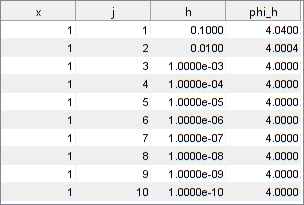
\includegraphics[scale=1]{cap1/es3.png}
\end{center}

Questi risultati verificano che, per valori sufficientemente piccoli di \(h\), il rapporto incrementale \(\phi_h(x) \approx f'(x)\) in quanto \(f'(x) = 4x^3\).

\vspace{1cm}
\subsection{\textbf{Esercizio 4}}
\vspace{0.5cm}
%\begin{center}
\footnotesize\noindent\fbox{
	\parbox{\textwidth}{
	 Si dia una maggiorazione del valore assoluto dell'errore relativo con cui \(x+y+z\) viene approssimato dall'approssimazione prodotta dal calcolatore, ossia \((x \oplus y) \oplus z\) (supporre che non ci siano problemi di overflow o di underflow). Ricavare l'analoga maggiorazione anche per \(x \oplus (y \oplus z)\) tenendo presente che \(x \oplus (y \oplus z) = (y \oplus z) \oplus x \).
	}
}\end{center}

\noindent Si consideri la definizione dell'operazione somma in aritmetica di macchina e la si applichi al caso richiesto:

\begin{itemize}

\item \((x \oplus y) \oplus z = fl( fl( fl(x) + fl(y) ) + fl(z)) \)
\item \((y \oplus z) \oplus x = fl( fl( fl(y) + fl(z) ) + fl(x)) \)

\end{itemize}

\noindent Ricordando che \(fl(a) = a + a\varepsilon_a = a (1 + \varepsilon_a)\) e che \(|\varepsilon_a| \leq u\) con \(u\) precisione di macchina, possiamo ricavare:

\[
|\varepsilon_{(x \oplus y) \oplus z }| = \frac{|fl( fl( fl(x) + fl(y) ) + fl(z)) - (x + y + z)|}{|x+y+z|}
\]
\[=
\frac{|((x + x\varepsilon_x + y + y\varepsilon_y)(1+\varepsilon_{x \oplus y}) + z + z\varepsilon_z)(1 +\varepsilon_{(x \oplus y) \oplus z }) - (x+y+z)|}{|x+y+z|}
\]
\[
=\frac{\left|\splitfrac{x\varepsilon_x + y\varepsilon_y + x\varepsilon_{x \oplus y} + x\varepsilon_x\varepsilon_{x \oplus y} + y\varepsilon_{x \oplus y} + y\varepsilon_y\varepsilon_{x \oplus y} + z\varepsilon_z + x\varepsilon_x\varepsilon_{(x \oplus y) \oplus z} + y\varepsilon_y\varepsilon_{(x \oplus y) \oplus z}    }{     + x\varepsilon_{x \oplus y}\varepsilon_{(x \oplus y) \oplus z} + x\varepsilon_x\varepsilon_{x \oplus y}\varepsilon_{(x \oplus y) \oplus z} + y\varepsilon_{x \oplus y}\varepsilon_{(x \oplus y) \oplus z} + y\varepsilon_y\varepsilon_{x \oplus y}\varepsilon_{(x \oplus y) \oplus z} + z\varepsilon_z\varepsilon_{(x \oplus y) \oplus z}}\right|}{|x+y+z|}
\]
\[
\leq \frac{\left|\splitfrac{\max \{\varepsilon_x, \varepsilon_y, \varepsilon_z\}(2x+2y+z) }{  \splitfrac{+ \max \{\varepsilon_x, \varepsilon_y, \varepsilon_z, \varepsilon_{x \oplus y}, \varepsilon_{(x \oplus y) \oplus z}\} ^2 (3x+3y+z) }{+  \max \{\varepsilon_x, \varepsilon_y, \varepsilon_z, \varepsilon_{x \oplus y}, \varepsilon_{(x \oplus y) \oplus z}\} ^3 (x+y)}}\right|}{|x+y+z|}
\]

\noindent Data la natura dell'errore relativo, possiamo trascurare tutti i termini di gradi superiore al primo in quanto sensibilmente pi\'u piccoli di \(\max \{\varepsilon_x, \varepsilon_y, \varepsilon_z, \varepsilon_{x \oplus y}, \varepsilon_{(x \oplus y) \oplus z}\} \). Avremo quindi:
\[
|\varepsilon_{(x \oplus y) \oplus z }| \leq \max \{\varepsilon_x, \varepsilon_y, \varepsilon_z, \varepsilon_{x \oplus y}, \varepsilon_{(x \oplus y) \oplus z}\} \frac{|2x + 2y + z|}{|x+y+z|}
\]
\[
\leq u \frac{|2x + 2y + z|}{|x+y+z|}
\]
\\
\noindent Svolgendo un procedimento del tutto analogo al precedente, nel caso di \((y \oplus z) \oplus x \) avremo:

\[
\varepsilon_{(y \oplus z) \oplus x } \leq u \frac{|2y + 2z + x|}{|x+y+z|}
\]

\vspace{1cm}
\subsection{\textbf{Esercizio 5}}
\vspace{0.5cm}
%\lstinputlisting[language=Matlab]{cap1/es5_1-16.m}

\begin{tabular}{l*{6}{c}}
 x  &  count \\
\hline
 0.0625 & 1 \\
 0.1250 & 2 \\
 0.1875 & 3 \\
 0.2500 & 4 \\
 0.3125 & 5 \\
 0.3750 & 6 \\
 0.4375 & 7 \\
 0.5000 & 8 \\
 0.5625 & 9 \\
 0.6250 & 10 \\
 0.6875 & 11 \\
 0.7500 & 12 \\
 0.8125 & 13 \\
 0.8750 & 14 \\
 0.9375 & 15 \\
      1 & 16 \\
\end{tabular} \\

\noindent Il ciclo \(while\) esegue esattamente 16 iterazioni prima di fermarsi sulla condizione \(x \neq 1\), che viene meno nell'ultimo passo. Questo avviene ovviamente in accordo all'incremento di \(x\) pari a \(\frac{1}{16}\) ad ogni iterazione, dato che la rappresentazione binaria di del numero decimale \(\frac{1}{16} = 0.0625\) risulta esatta.
\\
\\
\noindent Eseguendo invece il seguente codice Matlab, il ciclo non termina.

\lstinputlisting[language=Matlab]{cap1/es5_1-20.m}

\begin{tabular}{l*{6}{c}}
 x  &  count \\
\hline
 0.050000000000000 & 1 \\
 0.100000000000000 & 2 \\
 0.150000000000000 & 3 \\
 0.200000000000000 & 4 \\
 0.250000000000000 & 5 \\
 0.300000000000000 & 6 \\
 0.350000000000000 & 7 \\
 \ldots & \ldots \\
 1.000000000000000 & 20 \\
 \ldots & \ldots \\
\end{tabular} \\

Dato che il valore di \(delta\) questa volta risulta uguale a \(\frac{1}{20} = 0.05\), la sua rappresentazione nel calcolatore non risulta esatta, quindi deve essere approssimato. L'errore di approssimazione della variabile \(delta\) si accumula ad ogni iterazione nella variabile \(x\). Essendo la condizione del ciclo \(while\) vincolata al raggiungimento del numero esatto \(1\), non viene mai verificata ed il ciclo continua indefinitamente.



\newpage
\section{\textbf{Capitolo 3}}
\vspace{0.8cm}
\subsection{\textbf{Esercizio 1}}
\begin{center}
\footnotesize\noindent\fbox{
	\parbox{\textwidth}{
	Scrivere una function Matlab per la risoluzione di un sistema lineare con matrice dei coefficienti triangolare inferiore a diagonale unitaria. Inserire un esempio di utilizzo.
	}
}\end{center}

\noindent Si veda il seguente codice Matlab:

\lstinputlisting[language=Matlab]{cap3/3_1.m}

\noindent La funzione realizzata risolve sistemi del tipo richiesto prendendo in input la matrice dei coefficienti \(A\) ed il vettore dei termini noti \(b\), restituendo il vettore delle soluzioni.
\\
\\
\noindent Nell'esempio risolto nel codice, il sistema in oggetto era questo:
\[
\begin{bmatrix}1 & 0 & 0 \\ 2 & 1 & 0\\ -1 & 2 & 1 \end{bmatrix} \vec{x} = \begin{bmatrix}1 \\ 2 \\ -2 \end{bmatrix}
\]
\noindent Il vettore delle soluzioni calcolato dalla funzione \'e, correttamente, \(\begin{bmatrix}1 \\ 0 \\ -1 \end{bmatrix}\).

\vspace{1cm}
\subsection{\textbf{Esercizio 2}}
\begin{center}
\footnotesize\noindent\fbox{
	\parbox{\textwidth}{
	Utilizzare l'Algoritmo 3.6 del libro per stabilire se le seguenti matrici sono sdp o no:

\[
A_1 = \begin{pmatrix}1 & -1 & 2 & 2 \\ -1&5&-14&2\\ 2&-14&42&2\\2&2&2&65 \end{pmatrix},
A_2 = \begin{pmatrix}1 & -1 & 2 & 2 \\ -1&6&-17&3\\ 2&-17&48&-16\\2&3&-16&4 \end{pmatrix}
\]
	}
}\end{center}

\noindent Il seguente codice Matlab implementa una versione dell'algoritmo 3.6 del libro e la utilizza per rispondere a quanto richeisto. Nel merito, la matrice \(A_1\) \'e simmetrica e definita positiva, mentre la matrice \(A_2\) non lo \'e.
\\

\lstinputlisting[language=Matlab]{cap3/3_2.m}

\vspace{1cm}
\subsection{\textbf{Esercizio 3}}
\begin{center}
\footnotesize\noindent\fbox{
	\parbox{\textwidth}{
	Scrivere una function Matlab che, avendo in ingresso un vettore b contenente i termini noti del sistema lineare \(Ax = b\) con \textit{A} sdp e l'output dell'Algoritmo 3.6 del libro (matrice \(A\) riscritta nella porzione triangolare inferiore con i fattori \(L\) e \(D\) della fattorizzazione \(LDL^T\) di \(A\)), ne calcoli efficientemente la soluzione.
	}
}\end{center}

\noindent Il seguente codice Matlab soddisfa la richiesta. Riguardo alla function \lstinline[language=Matlab]{sist_triang_inf}, la sua implementazione \'e quella dell'Esercizio 1.
\\
\lstinputlisting[language=Matlab]{cap3/3_3.m}

\noindent Si notino i seguenti aspetti del codice mostrato:
\begin{itemize}

\item il vettore delle soluzioni dei sottosistemi viene memorizzato nelle stesse locazioni di memoria del vettore dei termini noti avuto in input;
\item la scomposizione della matrice A nei suoi fattori L e D non viene memorizzata fisicamente in due matrici diverse, ma avviene nella stessa porzione di memoria occupata dalla sola matrice A.
\item gli algoritmi scelti per la risoluzione dei sistemi triangolari accedono entrambi agli elementi della matrice \textit{per colonne}, in accordo con il tipo di memorizzazione delle matrici prevista da Matlab.
\end{itemize}

\noindent Quindi, la soluzione proposta \'e efficiente sia per quanto riguarda l'occupazione di memoria che per la minimizzazione del tempo di input/output.

\vspace{1cm}
\subsection{\textbf{Esercizio 4}}
\begin{center}
\footnotesize\noindent\fbox{
	\parbox{\textwidth}{
	Scrivere una function Matlab che, avendo in ingresso un vettore \textbf{b} contenente i termini noti del sistema lineare \(Ax = b\)  e l'output dell'Algoritmo 3.7 del libro (matrice \(A\) riscritta con la fattorizzazione LU con pivoting parziale e il vettore \textbf{p} delle permutazioni), ne calcoli efficientemente la soluzione.
	}
}\end{center}

\noindent Il seguente codice Matlab soddisfa la richiesta. Riguardo alle function \lstinline[language=Matlab]{sist_triang_inf} e \lstinline[language=Matlab]{sist_triang_sup}, le loro implementazioni sono quelle degli Esercizi 1 e 3.
\\

\lstinputlisting[language=Matlab]{cap3/3_4.m}

\noindent Riguardo all'efficienza della soluzione proposta, valgono le stesse considerazioni espresse nell'Esercizio 3.

\vspace{1cm}
\subsection{\textbf{Esercizio 5}}
\begin{center}
\footnotesize\noindent\fbox{
	\parbox{\textwidth}{
	Inserire alcuni esempi di utilizzo delle due function implementate per i punti 3 e 4, scegliendo per ciascuno di essi un vettore \(\overline{x}\) e ponendo \(b = A\overline{x}\). Riportare \(\overline{x}\) e la soluzione \(x\) da essi prodotta. Costruire anche una tabella in cui, per ogni esempio considerato, si riportano il numero di condizionamento di A in norma 2 (usare \lstinline[language=Matlab]{cond} di Matlab) e le quantit\'a \(||r||/||b||\) e \(||x-\overline{x}||/||\overline{x}||\).
	}
}\end{center}

\noindent Si presenta di seguito un esempio per la function dell'Esercizio 3 (risoluzione di sistemi con scomposizione \(LDL^T\)) ed un esempio per la function dell'Esercizio 4 (scomposizione LU con pivoting parziale). La matrice scelta per entrambi gli esempi \'e la seguente:
\[
A = \begin{pmatrix} 1 & -1 & 2 & 2 \\ -1 & 5 & -14 & 2\\ 2 & -14 & 42 & 2\\ 2 & 2 & 2 & 65 \end{pmatrix}
\]

\noindent I vettori scelti sono, rispettivamente per gli Esercizi 3 e 4:

\[
\overline{x}_3 = \begin{bmatrix} 3.1416 \\ 2.7183 \\ 1.4142 \\ 1.7320 \end{bmatrix},
\overline{x}_4 = \begin{bmatrix} 2.2360 \\ 2.6457 \\ 3.1416 \\ 3.3166 \end{bmatrix}
\]

\noindent Ponendo \(b=A\overline{x}\) si ha quindi:
\\
\[
b_3 = \begin{bmatrix} 6.7157 \\ -5.8849 \\ 31.0874 \\ 127.1282 \end{bmatrix},
b_4 = \begin{bmatrix} 12.5067 \\ -26.3567 \\ 106.0126 \\ 231.6256 \end{bmatrix}
\]

\noindent Lanciando le opportune function per la preparazione delle matrici e per la risoluzione del sistema (come mostrato nel dettaglio nel codice Matlab in coda a questa spiegazione), vengono prodotti i seguenti vettori soluzione:

\[
x_3 = \begin{bmatrix} 3.141600000000039 \\ 2.718300000000078 \\ 1.41420000000002 \\ 1.73200000000000 \end{bmatrix},
x_4 = \begin{bmatrix} 2.23599999999992 \\ 2.64569999999982 \\ 3.14159999999994 \\ 3.31660000000001 \end{bmatrix}
\]
\\
\noindent A seguire la tabella richiesta, che mostra il condizionamento della matrice restituita dagli algoritmi di fattorizzazione e le quantit\'a richieste, analoghe ad errori relativi sui dati di ingresso (\(||r||/||b||\)) e sul risultato (\(||x-\overline{x}||/||\overline{x}||\)).
\\

\noindent\begin{tabular}{l*{20}{c}}
function & \vline& tipo & \vline& \(\overline{x}\) & \vline& \(cond(A, 2)\) & \vline& \(||r||/||b||\) & \vline& \(||x-\overline{x}||/||\overline{x}||\) \\
\hline
sol\_es\_3 & \vline& \(LDL^T\)    & \vline& \(\overline{x}_3\) & \vline& \(3.6158 \times 10^3\)    & \vline& \(1.1782 \times 10^{-32}\)	& \vline& \(3.6725 \times 10^{-28}\)   \\
sol\_es\_4 & \vline& \(LU\) pivot & \vline& \(\overline{x}_4\) & \vline& 319.10                    & \vline& \(1.4448 \times 10^{-32}\)	& \vline& \(1.2850 \times 10^{-27}\) 	 \\

\end{tabular}
\\
\\

\noindent Il codice Matlab usato per realizzare i precedenti esempi \'e il seguente. Le function riferite nel codice per le quali non \'e riportata l'implementazione sono quelle impiegate per risolvere gli esercizi precedenti.
\lstinputlisting[language=Matlab]{cap3/3_5.m}

\vspace{1cm}
\subsection{\textbf{Esercizio 6}}
\begin{center}
\footnotesize\noindent\fbox{
	\parbox{\textwidth}{
	Sia \(A = \begin{pmatrix} \epsilon & 1 \\ 1 & 1 \end{pmatrix}\) con \(\epsilon=10^{-13}\).  Definire L triangolare inferiore a diagonale unitaria e U diagonale superiore in modo che il prodotto LU sia la fattorizzazione LU di A e, posto \(b=Ae\) con \(e=(1,1)^{T}\), confrontare l'accuratezza della soluzione che si ottiene usando il comando \(U \ (L \ b)\) (Gauss senza pivoting) e il comando \(A \ b\) (Gauss con pivoting).
	}
}\end{center}


%...
\vspace{1cm}
\subsection{\textbf{Esercizio 10}}
\begin{center}
\footnotesize\noindent\fbox{
	\parbox{\textwidth}{
	Scrivere una function Matlab che realizza il metodo di Newton per un sistema nonlineare (prevedere un numero massimo di iterazioni e utilizzare il criteri di arresto basato sull'incremento in norma euclidea). Utilizzare la function costruita al punto 4 per la risoluzione del sistema lineare ad ogni iterazione.
	}
}\end{center}

\noindent Il seguente codice Matlab mostra l'implementazione della funzione richiesta. \'E stato necessario usare, oltre alla function costruita nell'Esercizio 4, anche l'implementazione dell'algoritmo 3.7 mostrata nell'Eserczio 5.
\\
\lstinputlisting[language=Matlab]{cap3/3_10.m}



\newpage
\section{\textbf{Capitolo 4}}
\vspace{0.8cm}
\subsection{\textbf{Esercizio 1}}
\begin{center}
\footnotesize\noindent\fbox{
	\parbox{\textwidth}{
	Scrivere una function Matlab che implementi il calcolo del polinomio interpolante di grado \textit{n} in forma di Lagrange. \\ \\La forma della function deve essere del tipo: \lstinline[language=Matlab]{y = lagrange( xi, fi, x)}
	}
}\end{center}

\newpage
\subsection{\textbf{Esercizio 2}}
\begin{center}
\footnotesize\noindent\fbox{
	\parbox{\textwidth}{
	Scrivere una function Matlab che implementi il calcolo del polinomio interpolante di grado \textit{n} in forma di Newton. \\ \\La forma della function deve essere del tipo: \lstinline[language=Matlab]{y = newton( xi, fi, x)}
	}
}\end{center}

\noindent Il seguente codice Matlab implementa la function richiesta. Si noti che, analogamente a quanto fatto per l'esercizio precedente, \'e stata realizzata una sottofunzione che implementa il calcolo delle differenze divise, al fine di rendere il codice pi\'u chiaro. \\ \\
\noindent \'E stata anche in questo caso calcolata un'interpolazione di esempio, per verificare la correttezza di quanto fatto.

\lstinputlisting[language=Matlab]{cap4/4_2.m}

\newpage
\subsection{\textbf{Esercizio 3}}
\begin{center}
\footnotesize\noindent\fbox{
	\parbox{\textwidth}{
	Scrivere una function Matlab che implementi il calcolo del polinomio interpolante di Hermite. \\ \\La forma della function deve essere del tipo: \lstinline[language=Matlab]{y = hermite( xi, fi, f1i, x)}
	}
}\end{center}


\noindent Il seguente codice Matlab implementa la function richiesta. Rimangono valide le stesse considerazioni espresse per gli esercizi precedenti.

\lstinputlisting[language=Matlab]{cap4/4_3.m}

\newpage
\subsection{\textbf{Esercizio 4}}
\begin{center}
\footnotesize\noindent\fbox{
	\parbox{\textwidth}{
	Utilizzare le functions degli esercizi precedenti per disegnare l'approssimazione della funzione \(\sin(x)\) nell'intervallo \([0, 2\pi]\), utilizzando le ascisse di interpolazione \(x_i=i\pi\), \(i=0,1,2\).
	}
}\end{center}

\newpage
\subsection{\textbf{Esercizio 5}}
\begin{center}
\footnotesize\noindent\fbox{
	\parbox{\textwidth}{
	Scrivere una function Matlab che implementi la spline cubica interpolante (naturale o \textit{not-a-knot}, come specificato in ingresso) delle coppie di dati assegnate. \\ \\La forma della funcion deve essere del tipo: \lstinline[language=Matlab]{y = spline3(xi, fi, x, tipo)}
	}
}\end{center}


\newpage
\subsection{\textbf{Esercizio 6}}
\begin{center}
\footnotesize\noindent\fbox{
	\parbox{\textwidth}{
	Scrivere una function Matlab che implementi il calcolo delle ascisse di Chebyshev per il polinomio interpolante di grado \textit{n}, su un generico intervallo \([a, b]\). \\ \\La function deve essere del tipo: \lstinline[language=Matlab]{ xi = ceby(n, a, b)}
	}
}\end{center}

\noindent Il seguente codice Matlab implementa la function richiesta. Si noti che la trasformazione lineare delle ascisse di Chebyshev dall'intervallo \([-1, 1]\) all'intervallo dato \([a, b]\) avviene direttamente come parte del calcolo delle stesse, evitando di scorrere il vettore in seguito con un altro ciclo, aumentando quindi l'efficienza della function. \\

\lstinputlisting[language=Matlab]{cap4/4_6.m}

\newpage
\subsection{\textbf{Esercizio 7}}
\begin{center}
\footnotesize\noindent\fbox{
	\parbox{\textwidth}{
	Utilizzare le function degli Esercizi 4.1 e 4.6 per graficare l'approssimazione della funzione di Runge sull'intervallo \([-6, 6]\), per \(n = 2, 4, 6, \ldots, 40\). \\ \\Stimare numericamente l'errore commesso in funzione del grado \textit{n} del polinomio interpolante.
	}
}\end{center}

\noindent Di seguito i grafici che mostrano i polinomi interpolanti di grado \textit{n} calcolati usando come punti di interpolazione quelli corrispondenti alle \textit{n} ascisse di Chebyshev (evidenziati in rosso), sovraimposti al grafico della funzione di Runge \(f(x) = \frac{1}{1+x^2}\) (in blu). \\

\noindent\small\begin{tabular}{l*{5}{c}}
\hspace{3.5cm}\(n=2\) & \(n=4\) \\
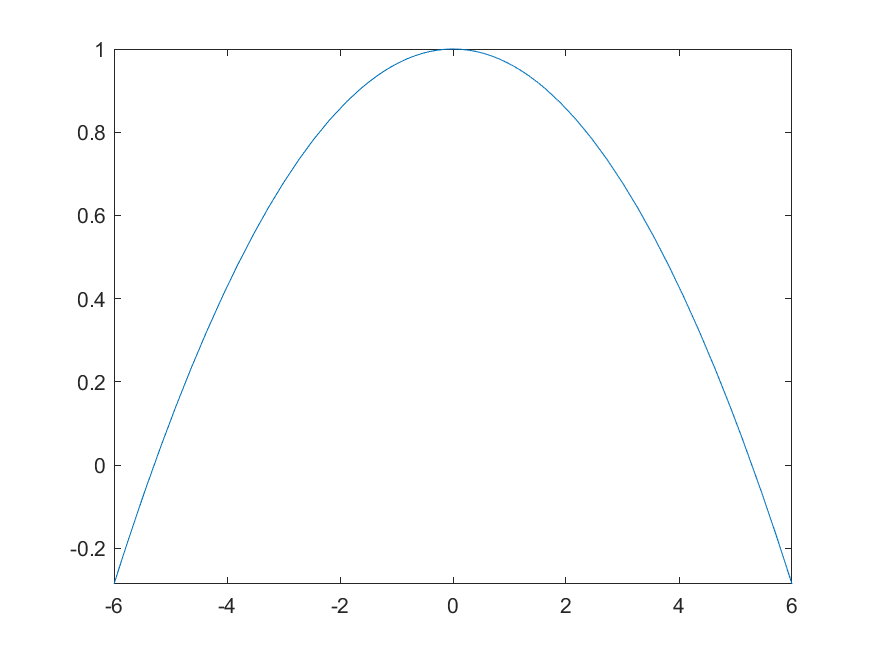
\includegraphics[scale=0.5]{cap4/4_7/2.png} &  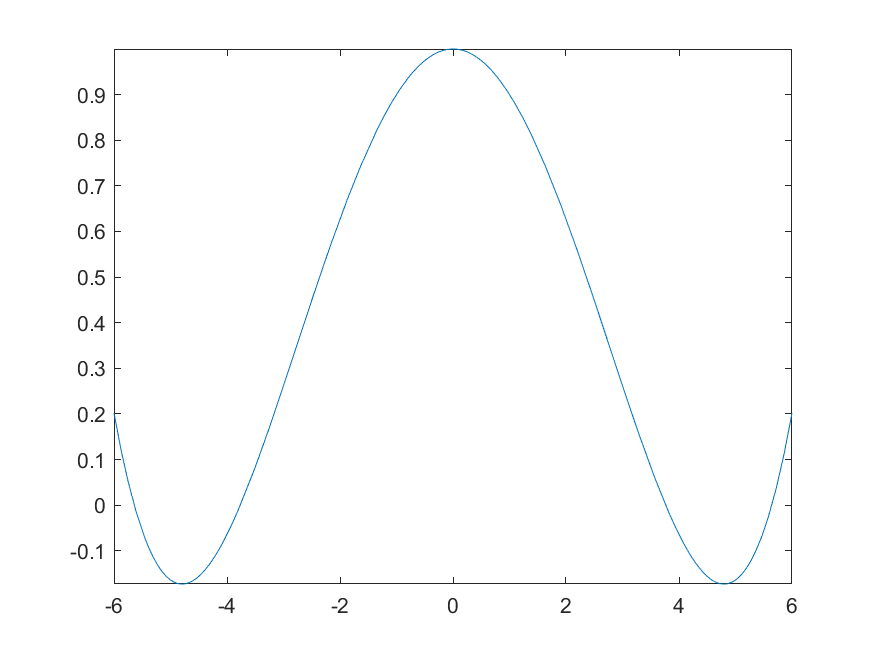
\includegraphics[scale=0.5]{cap4/4_7/4.png} \\

\hspace{3.5cm}\(n=6\)& \(n=8\) \\
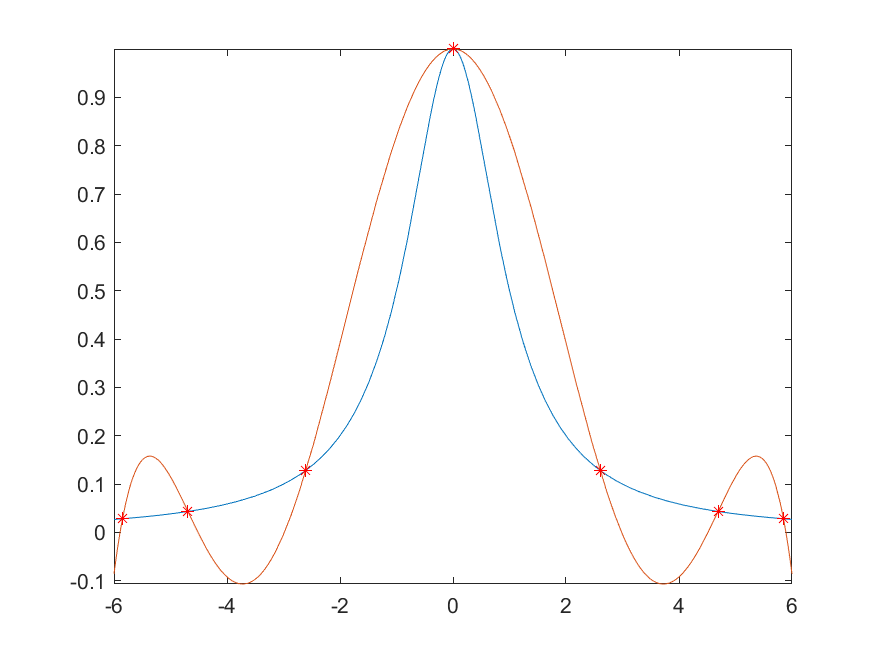
\includegraphics[scale=0.5]{cap4/4_7/6.png} &  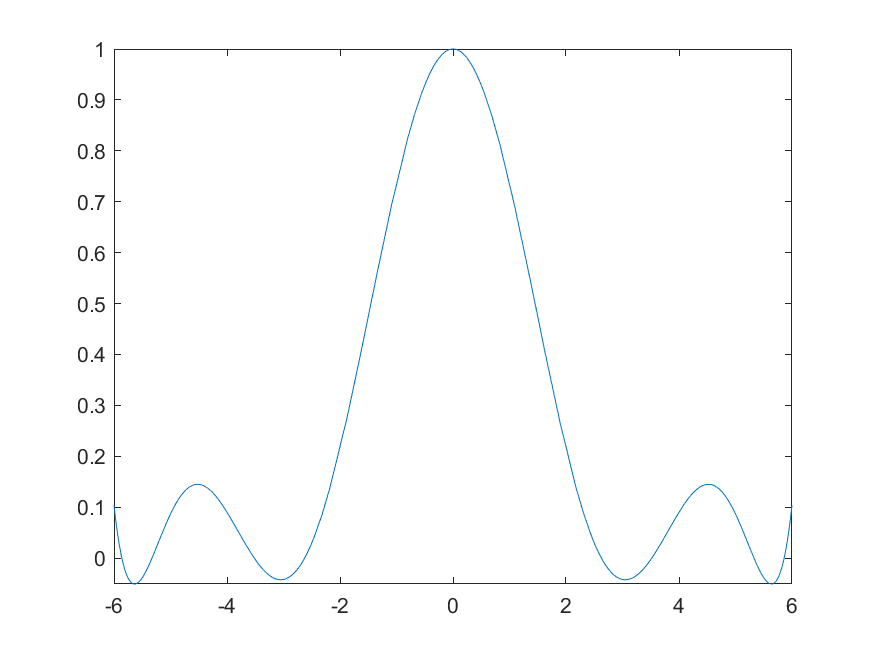
\includegraphics[scale=0.5]{cap4/4_7/8.png} \\

\hspace{3.5cm}\(n=10\) &  \(n=12\) \\
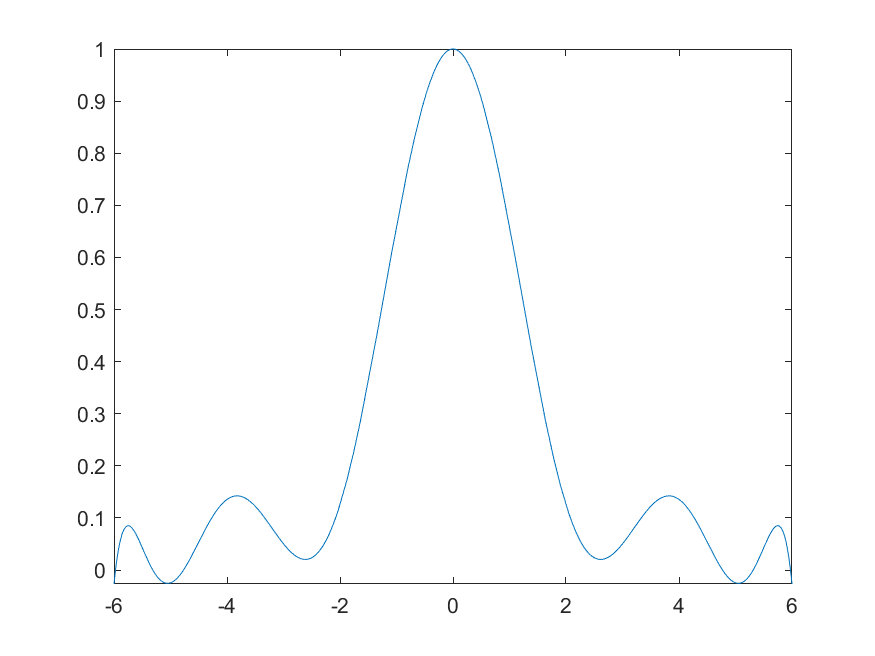
\includegraphics[scale=0.5]{cap4/4_7/10.png} &  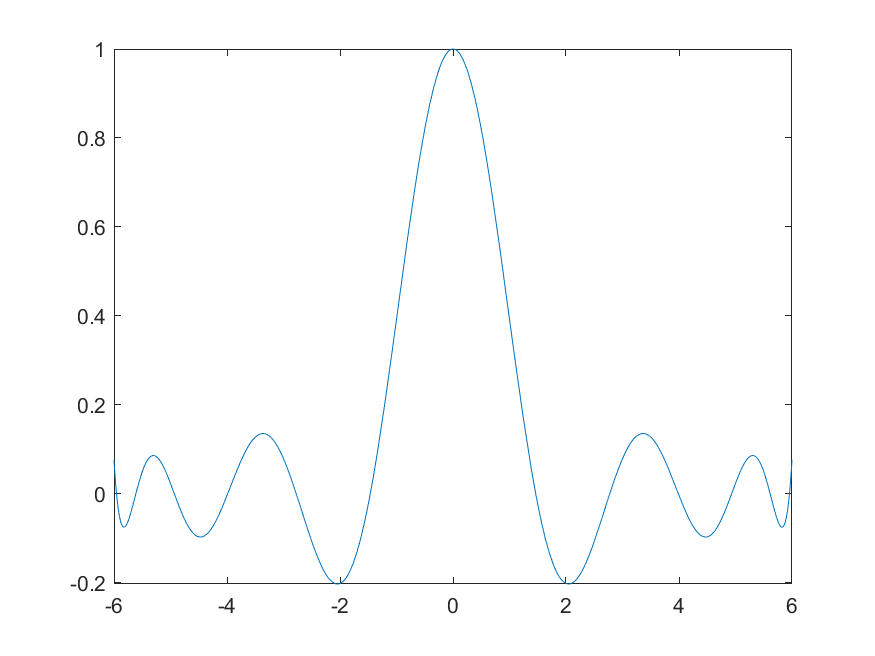
\includegraphics[scale=0.5]{cap4/4_7/12.png} \\
\end{tabular} \\ \\

\small\begin{tabular}{l*{5}{c}}
\hspace{3.5cm}\(n=14\) &  \(n=16\) \\
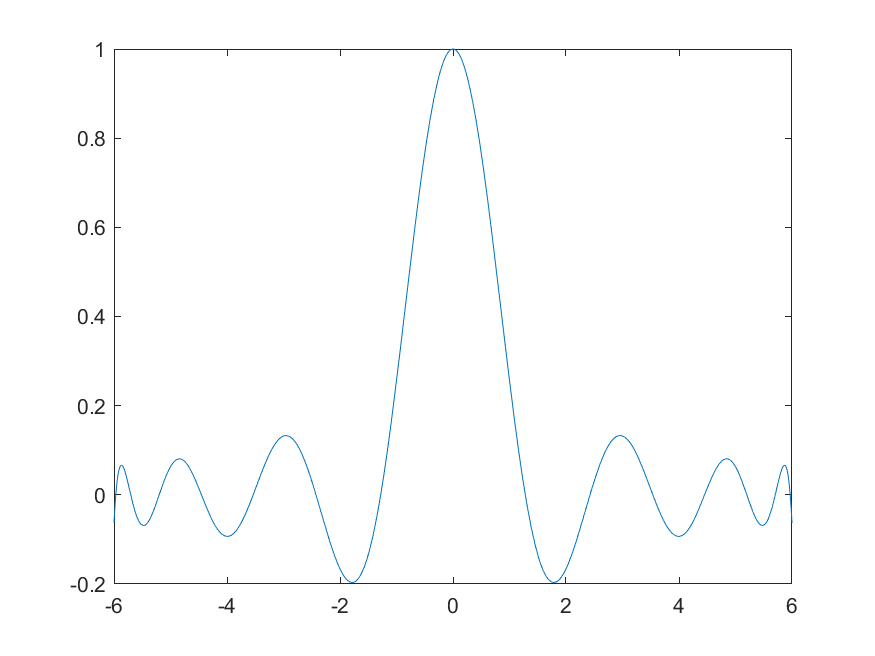
\includegraphics[scale=0.5]{cap4/4_7/14.png} &  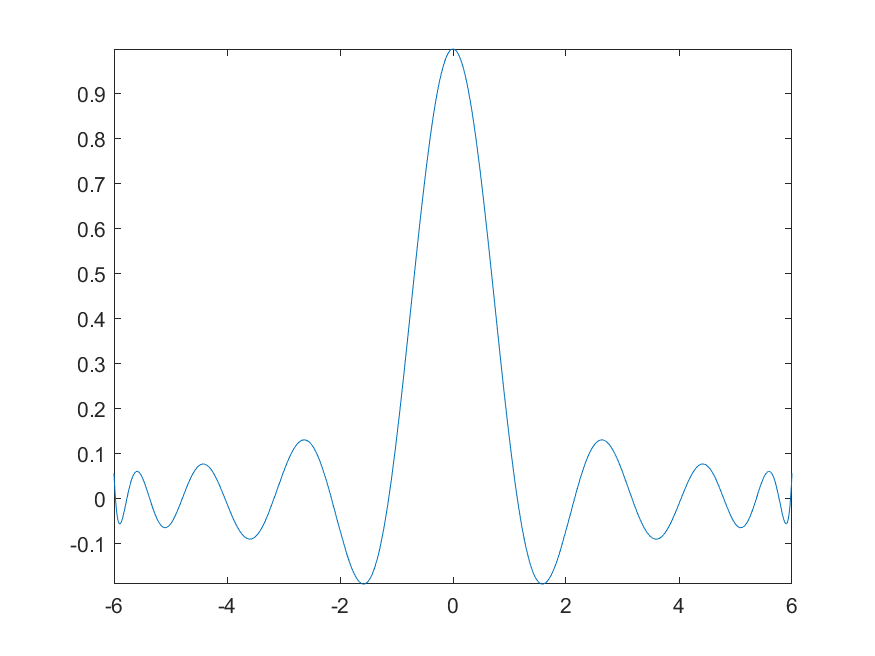
\includegraphics[scale=0.5]{cap4/4_7/16.png} \\

\hspace{3.5cm}\(n=18\) &  \(n=20\) \\
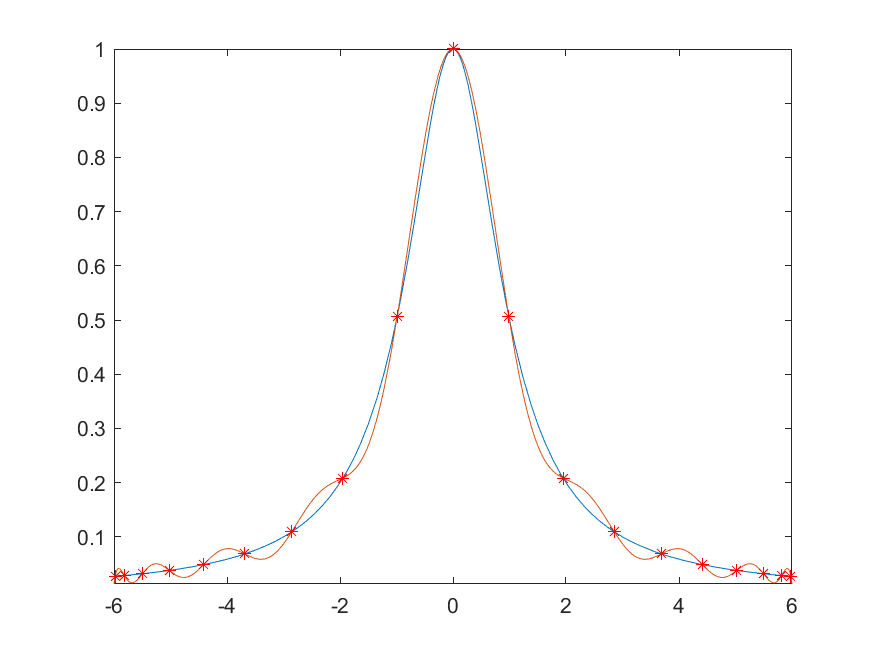
\includegraphics[scale=0.5]{cap4/4_7/18.png} &  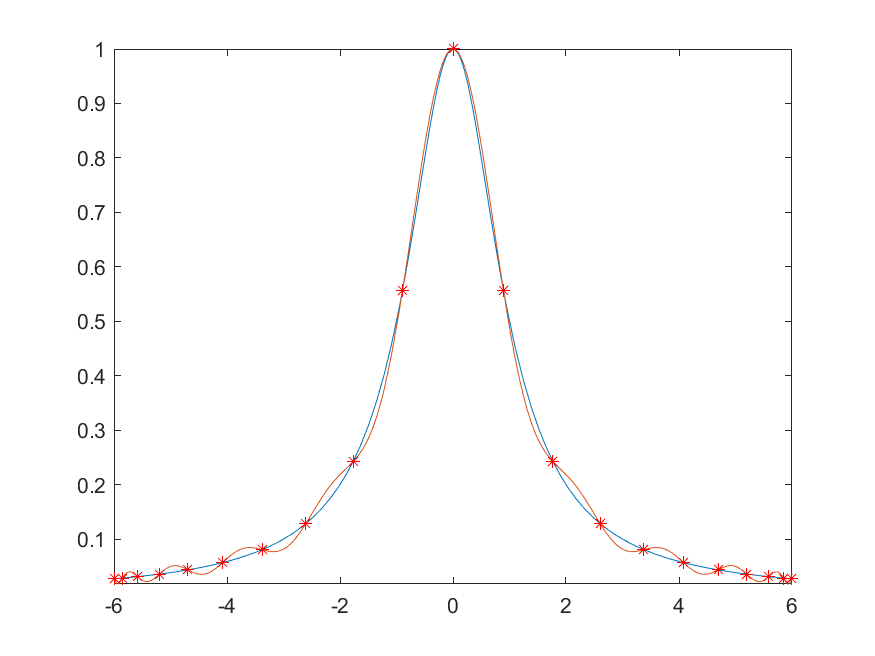
\includegraphics[scale=0.5]{cap4/4_7/20.png} \\

\hspace{3.5cm}\(n=22\) &  \(n=24\) \\
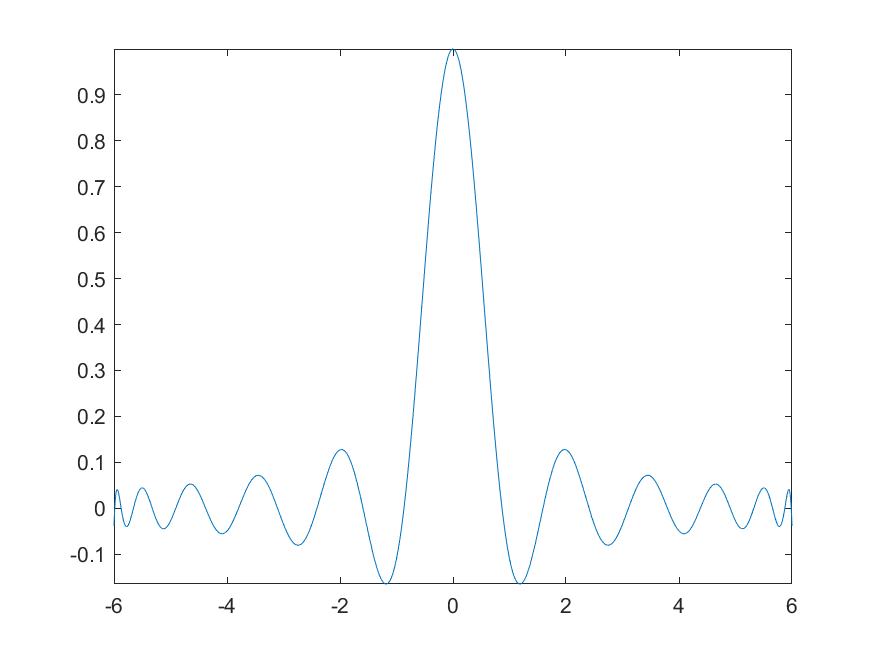
\includegraphics[scale=0.5]{cap4/4_7/22.png} &  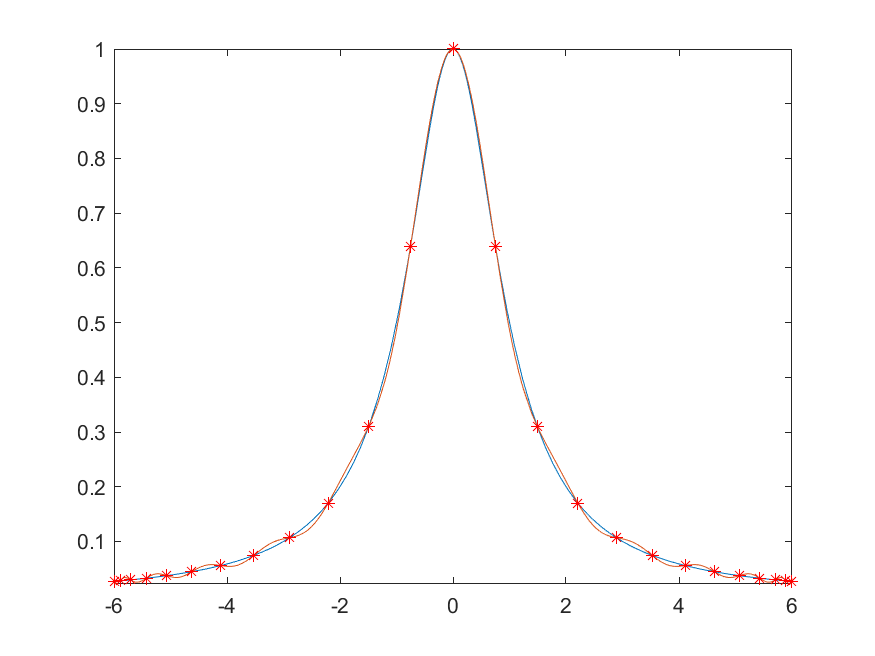
\includegraphics[scale=0.5]{cap4/4_7/24.png} \\

\hspace{3.5cm}\(n=26\) &  \(n=28\) \\
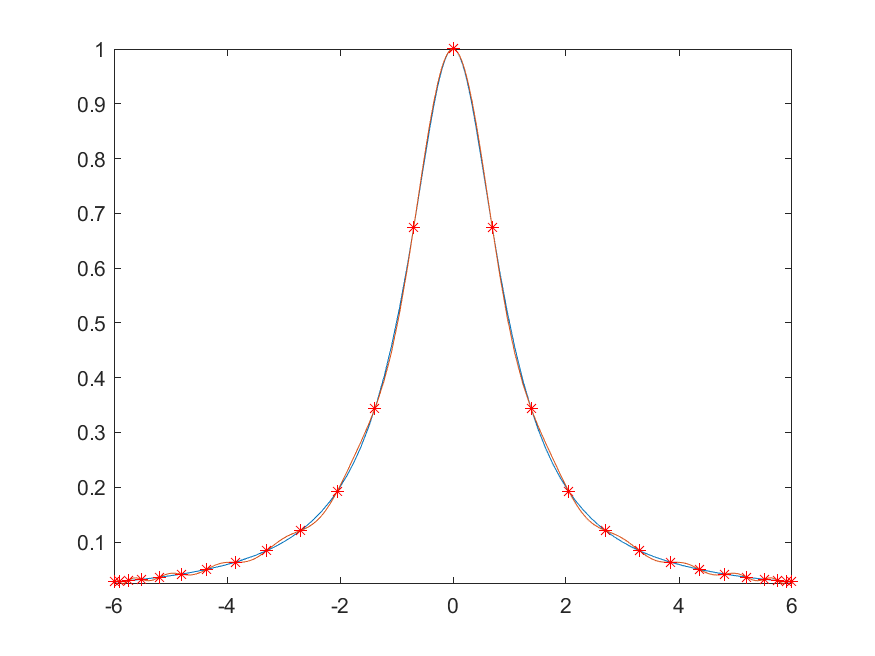
\includegraphics[scale=0.5]{cap4/4_7/26.png} &  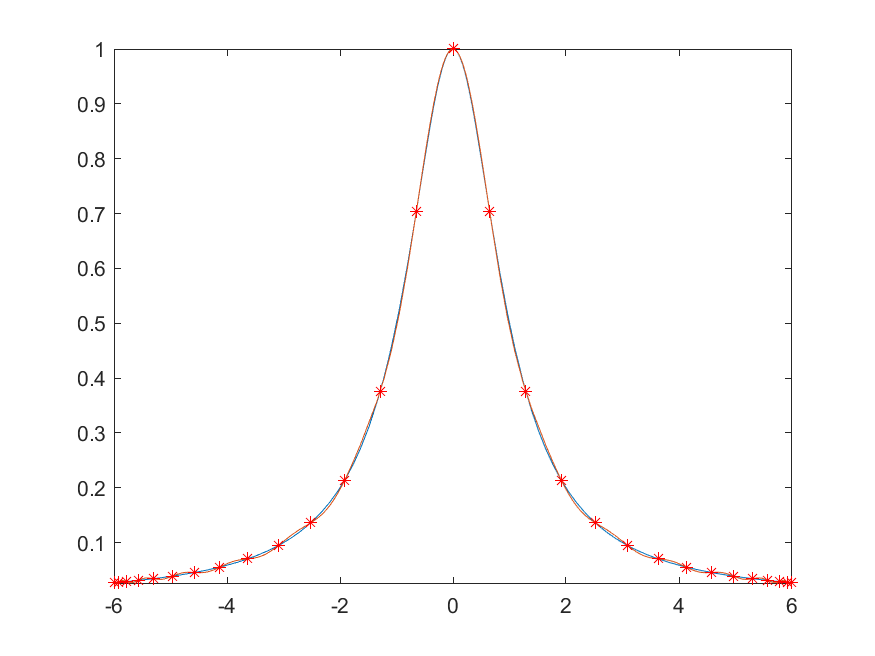
\includegraphics[scale=0.5]{cap4/4_7/28.png} \\
\end{tabular}

\small\begin{tabular}{l*{5}{c}}
\hspace{3.5cm}\(n=30\) &  \(n=32\) \\
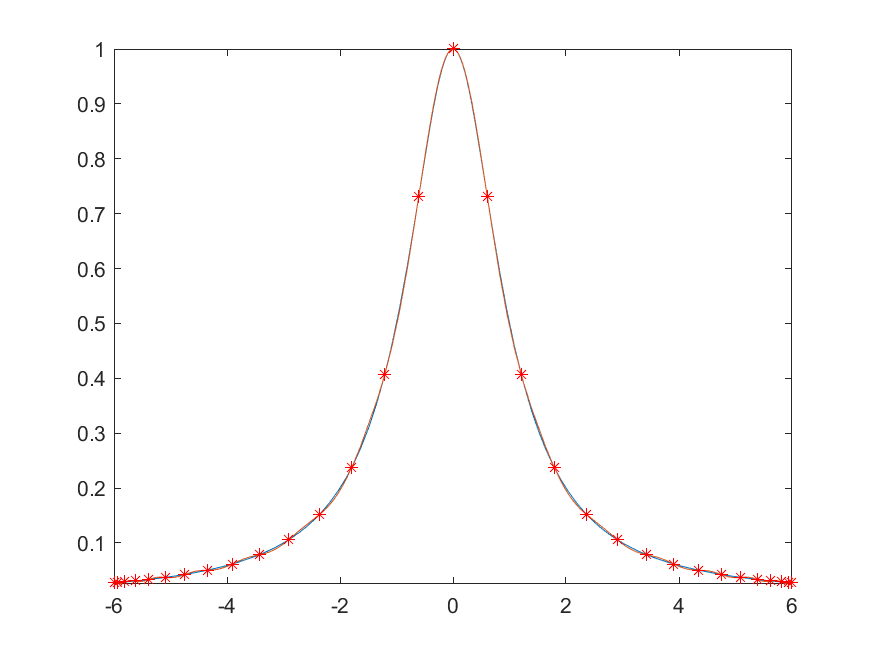
\includegraphics[scale=0.5]{cap4/4_7/30.png} &  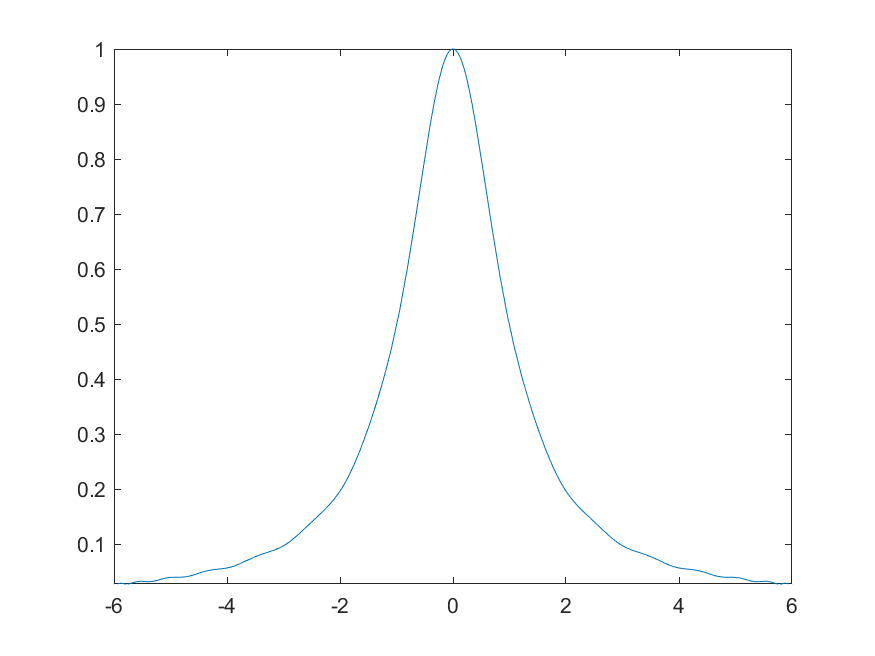
\includegraphics[scale=0.5]{cap4/4_7/32.png} \\

\hspace{3.5cm}\(n=34\) &  \(n=36\) \\
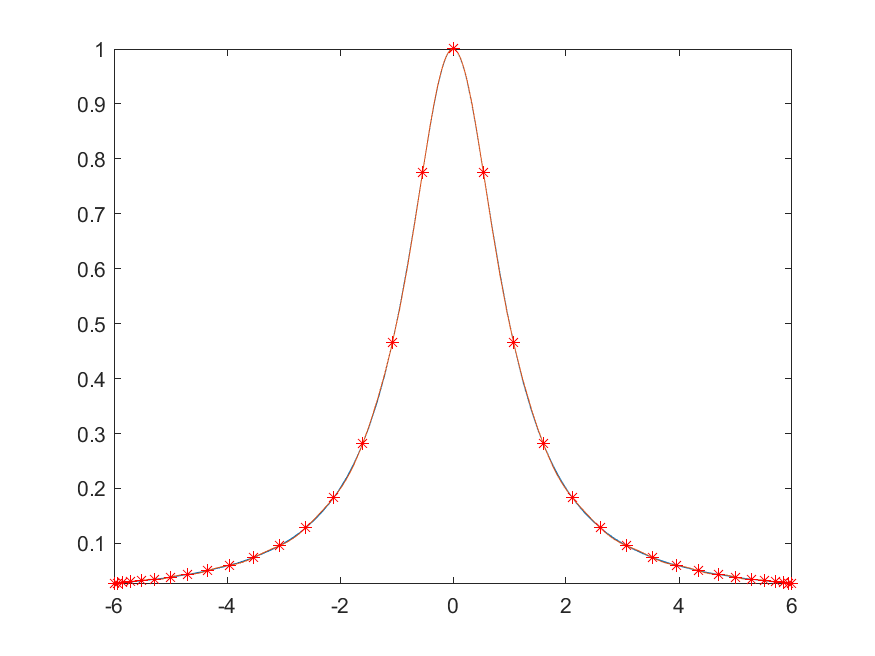
\includegraphics[scale=0.5]{cap4/4_7/34.png} &  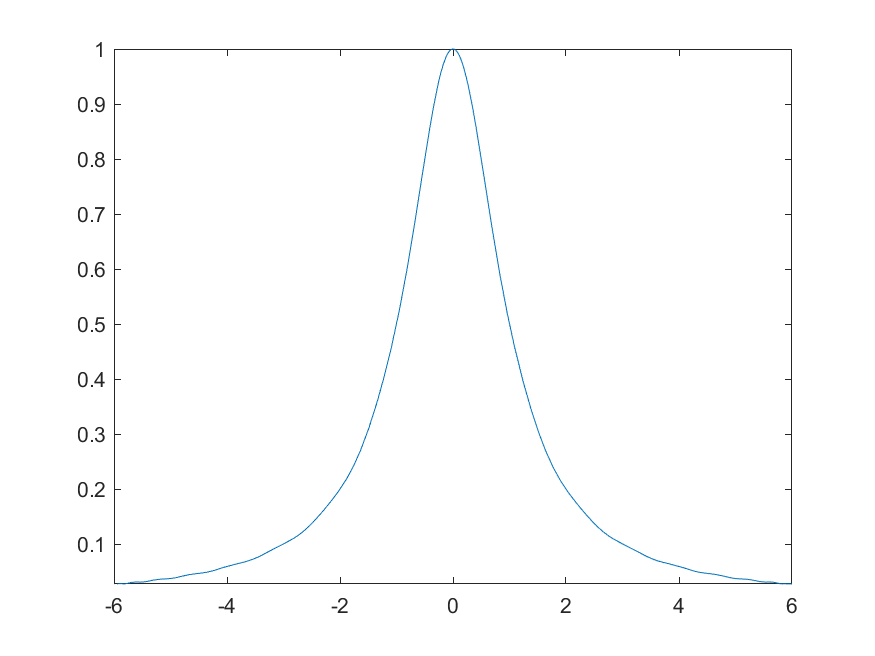
\includegraphics[scale=0.5]{cap4/4_7/36.png} \\

\hspace{3.5cm}\(n=38\) &  \(n=40\) \\
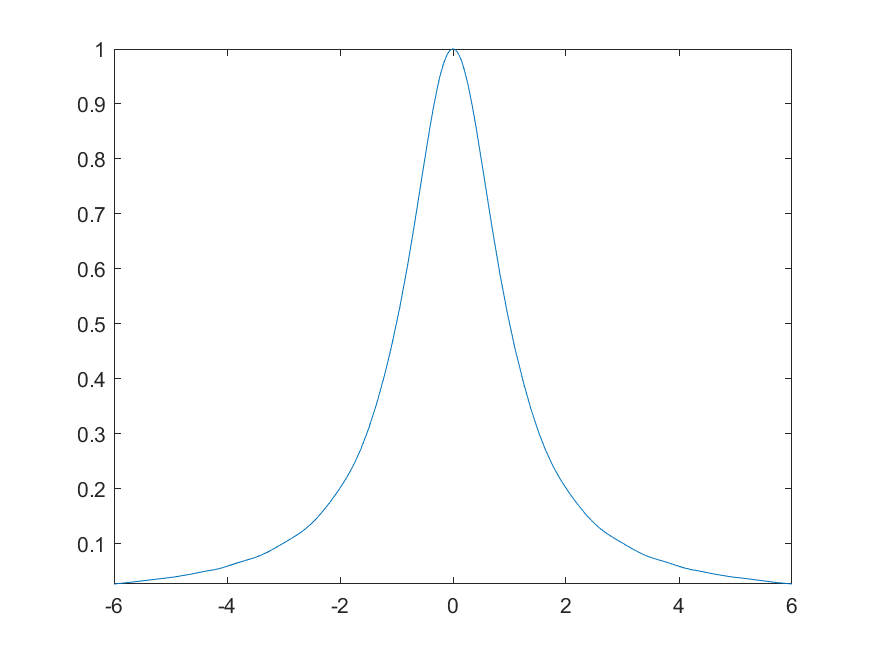
\includegraphics[scale=0.5]{cap4/4_7/38.png} &  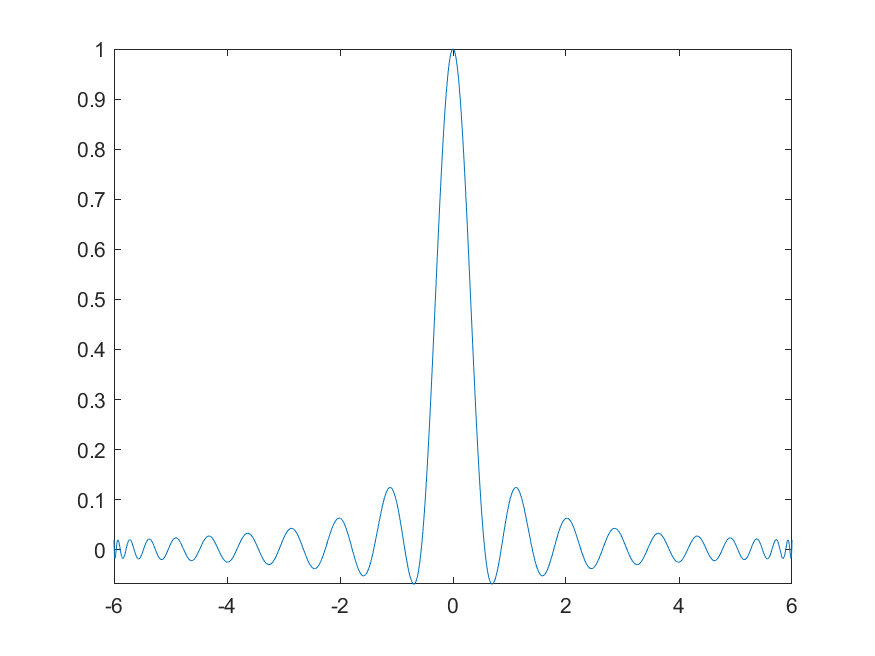
\includegraphics[scale=0.5]{cap4/4_7/40.png} \\
& \\
& \\
\end{tabular}


\noindent Riguardo all'errore commesso, grazie alla scelta dei nodi di Chebyshev come punti di interpolazione, per funzioni sufficientemente regolari abbiamo:
\[
||e|| \leq \frac{||f^{(n+1)}||}{(n+1)!2^n}
\]

\noindent Tuttavia, calcolare le derivate di ordine elevato della funzione di Runge risulterebbe molto dispendioso in termini computazionali. Quindi, ricaveremo una stima dell'errore in funzione di $n$ calcolandolo nel modo seguente:

$$
||e|| \approx ||f(x) - p_n(x)||_{\inf}
$$

\noindent con ovviamente $f$ intesa come la funzione di Runge e $p$ il suo polinomio interpolante.

\noindent L'errore così stimato è mostrato nella seguente tabella:

\begin{center}
	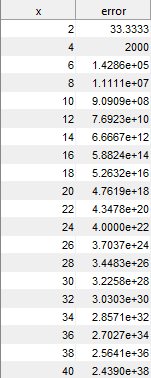
\includegraphics[scale=0.7]{cap4/4_7/4_7_error.png}
\end{center}

\noindent Come si pu\'o facilmente vedere, grazie alla scelta delle ascisse di Chebyshev come punti di interpolazione, l'errore diminuisce all'aumentare di \(n\), tendendo infatti a \(0\) per \(n \to \inf\).\\

\noindent Inoltre, \'e stato realizzato il seguente grafico mostrante l'andamento dell'errore nella parte destra dell'intervallo. La parte destra \'e stata omessa in quanto l'andamento dell'errore di interpolazione \'e simmetrico rispetto all'asse dellle ordinate: questo ha permesso di aumentare il livello di dettaglio del grafico, migliorandone la chiarezza e la visibilità.

\begin{center}
	\includegraphics[scale=0.7]{cap4/4_7/4_9_error.png}
\end{center}

\noindent Il codice Matlab con cui sono stati realizzati i grafci e la tabella mostrati sopra \'e il seguente: \\

\lstinputlisting[language=Matlab]{cap4/4_7.m}

\newpage
\subsection{\textbf{Esercizio 8}}
\begin{center}
\footnotesize\noindent\fbox{
	\parbox{\textwidth}{
	Relativamente al precedente esercizio, stimare numericamente la crescita della costante di Lebesgue.
	}
}\end{center}

\noindent Essendo le ascisse di interpolazione i nodi di Chebyshev, la costante di Lebesgue in fuzione di \(n\) si comporta come segue:
\[
\Lambda_n \approx \frac{2}{\pi}\log n
\]

\noindent Ci si aspetta quindi che abbia una crescita logaritmica al crescere di \(n\). Questo fatto \'e stato verificato calcolando le seguenti stime numeriche:

\begin{center}
	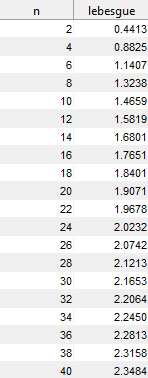
\includegraphics[scale=0.7]{cap4/4_8.png}
\end{center}

\noindent Il codice Matlab usato per realizzare la precedente tabella \'e il seguente:

\lstinputlisting[language=Matlab]{cap4/4_8.m}

\newpage
\subsection{\textbf{Esercizio 9}}
\begin{center}
\footnotesize\noindent\fbox{
	\parbox{\textwidth}{
	Utilizzare la function ell'Esercizio 4.1 per approssimare la funzione di Runge sull'intervallo \([-6, 6]\), su una partizione uniforme di \(n+1\) ascisse per \(n = 2, 4, 6, \ldots, 40\). Stimare le corrispondenti costanti di Lebesgue.
	}
}\end{center}

\noindent Di seguito i grafici che mostrano i polinomi interpolanti di grado \textit{n} calcolati usando come punti di interpolazione le ascisse equispaziate nell'intervallo \([-6, 6]\) (evidenziati in rosso), sovraimposti al grafico della funzione di Runge \(f(x) = \frac{1}{1+x^2}\) (in blu). \\


\noindent\small\begin{tabular}{l*{5}{c}}
\hspace{3.5cm}\(n=2\) & \(n=4\) \\
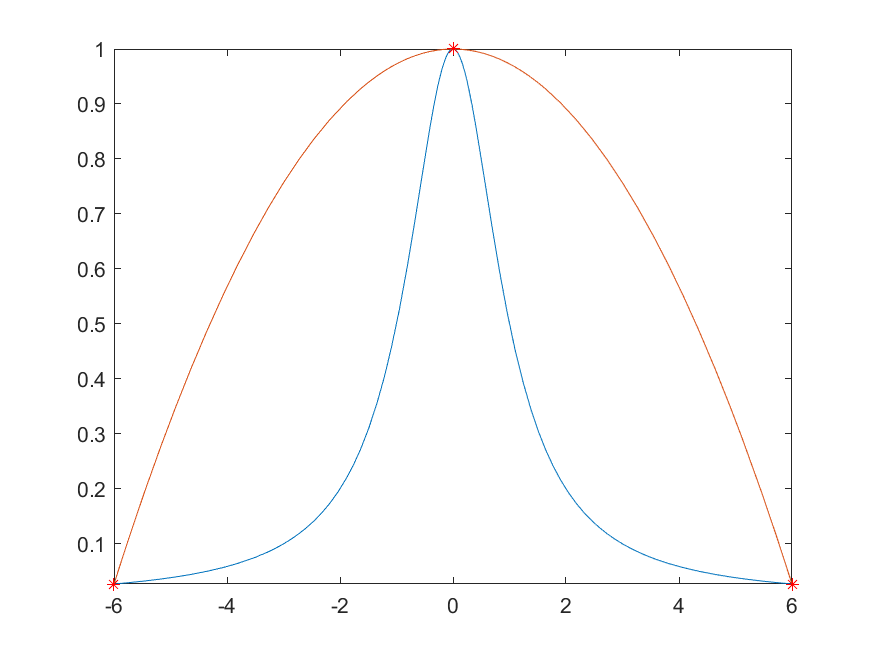
\includegraphics[scale=0.5]{cap4/4_9/2.png} &  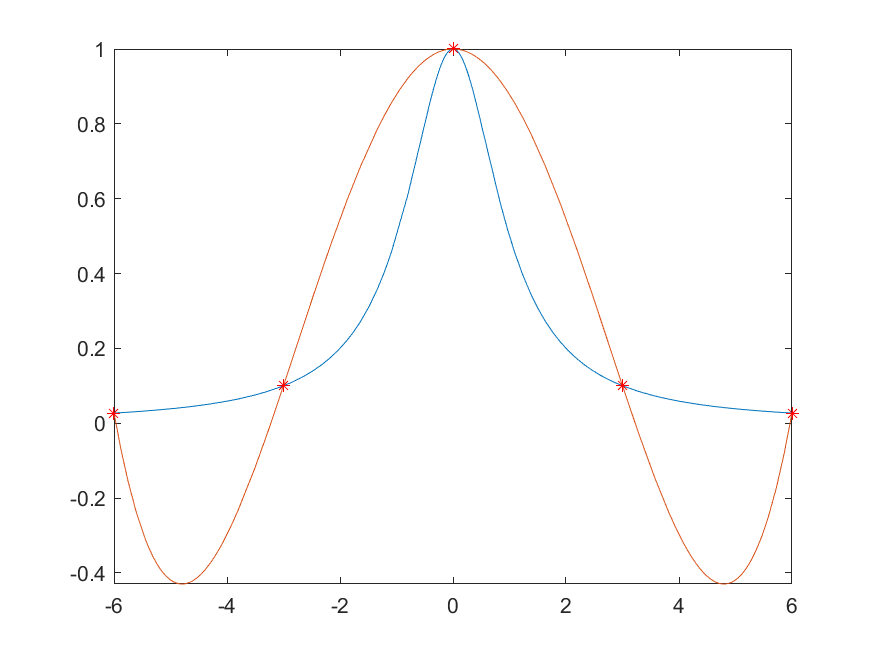
\includegraphics[scale=0.5]{cap4/4_9/4.png} \\

\hspace{3.5cm}\(n=6\)& \(n=8\) \\
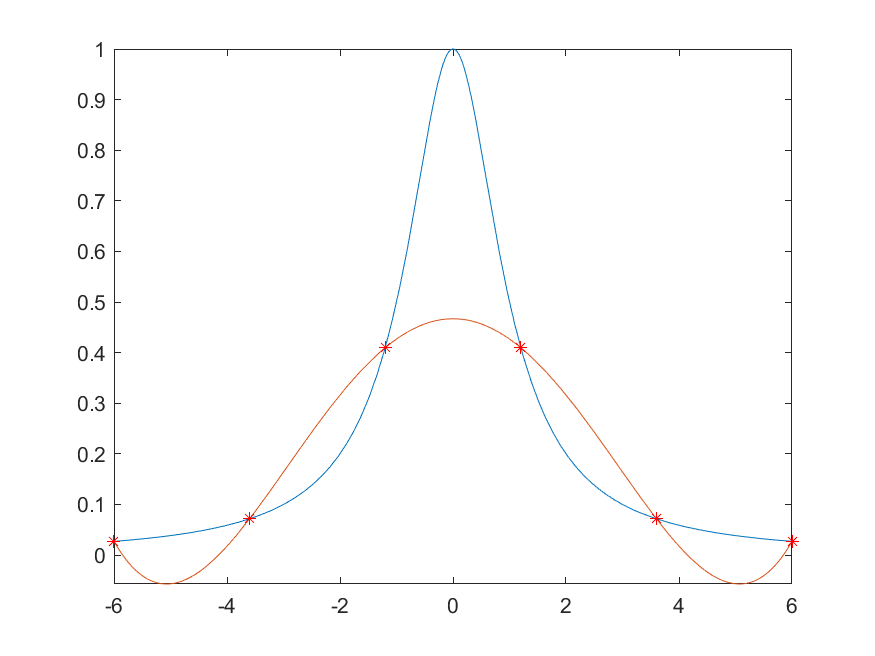
\includegraphics[scale=0.5]{cap4/4_9/6.png} &  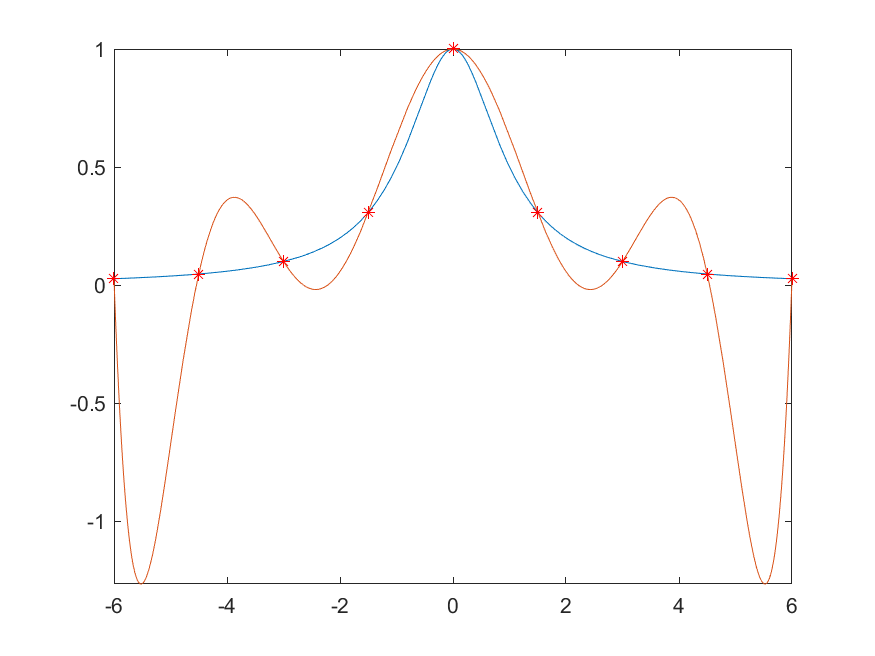
\includegraphics[scale=0.5]{cap4/4_9/8.png} \\

\hspace{3.5cm}\(n=10\) &  \(n=12\) \\
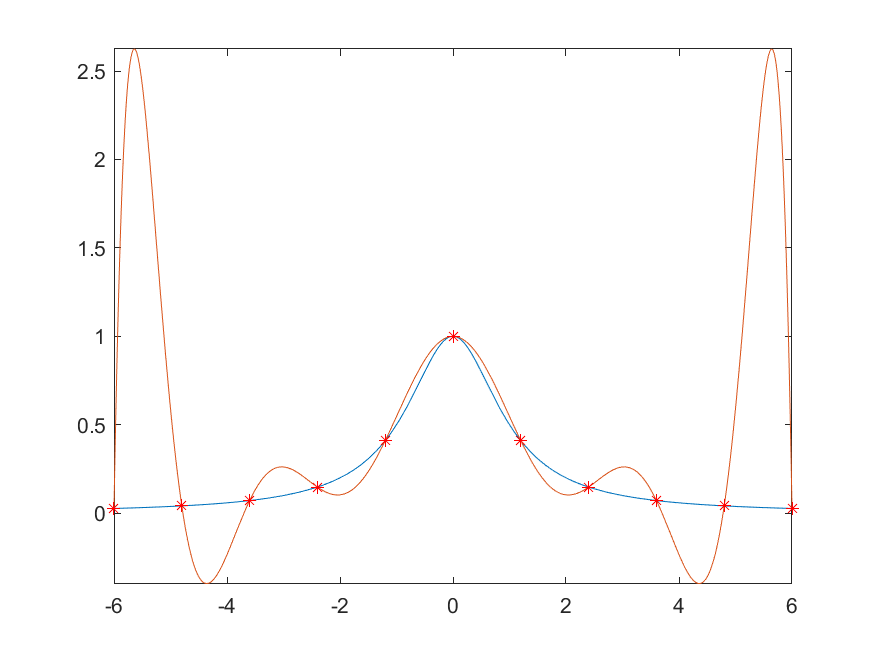
\includegraphics[scale=0.5]{cap4/4_9/10.png} &  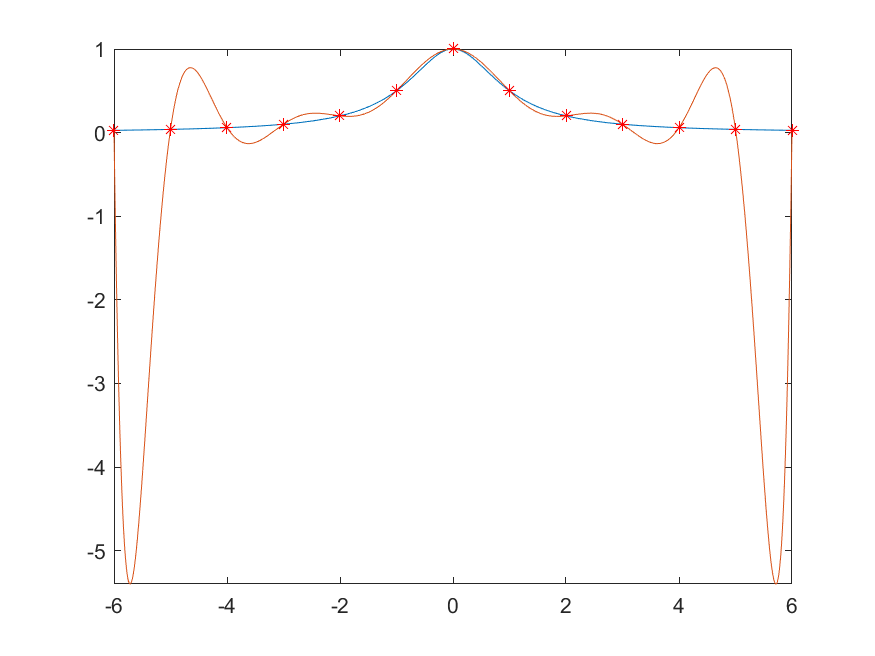
\includegraphics[scale=0.5]{cap4/4_9/12.png} \\
\end{tabular} \\ \\

\small\begin{tabular}{l*{5}{c}}
\hspace{3.5cm}\(n=14\) &  \(n=16\) \\
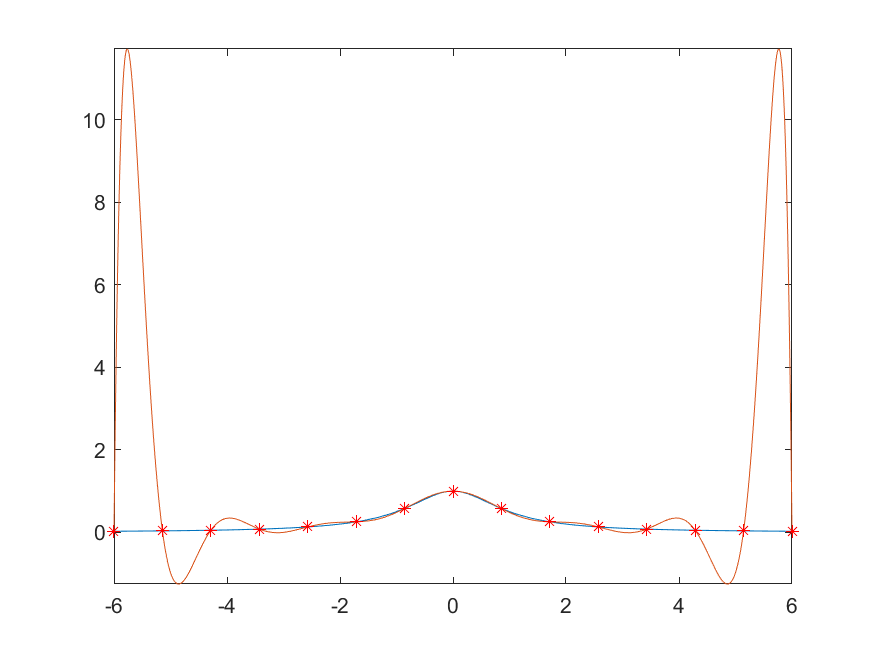
\includegraphics[scale=0.5]{cap4/4_9/14.png} &  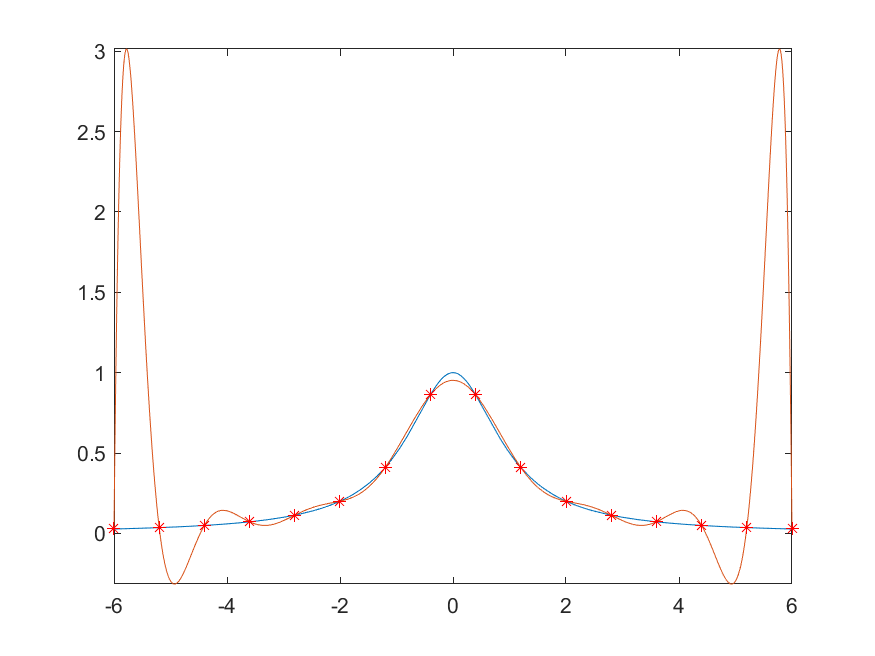
\includegraphics[scale=0.5]{cap4/4_9/16.png} \\

\hspace{3.5cm}\(n=18\) &  \(n=20\) \\
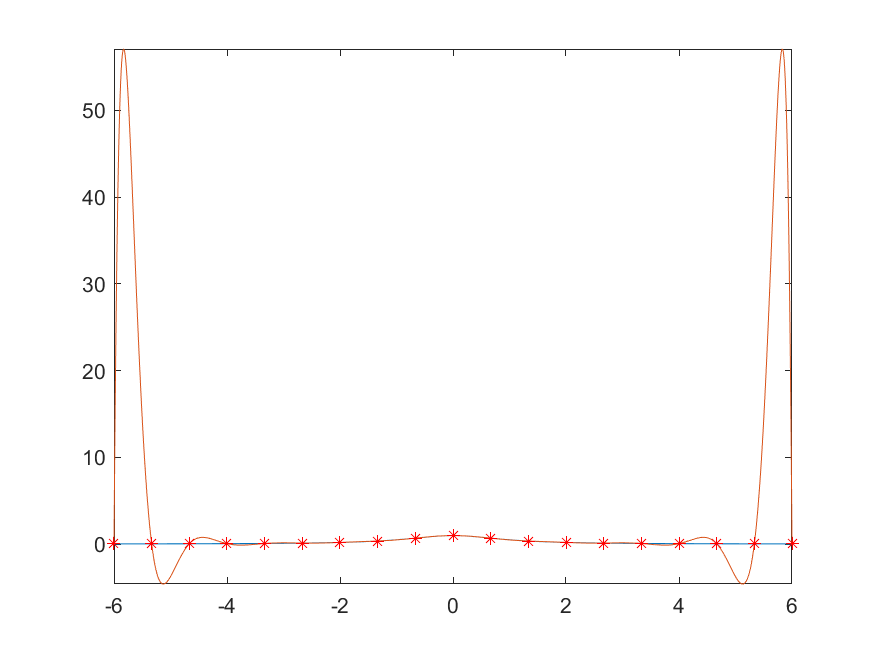
\includegraphics[scale=0.5]{cap4/4_9/18.png} &  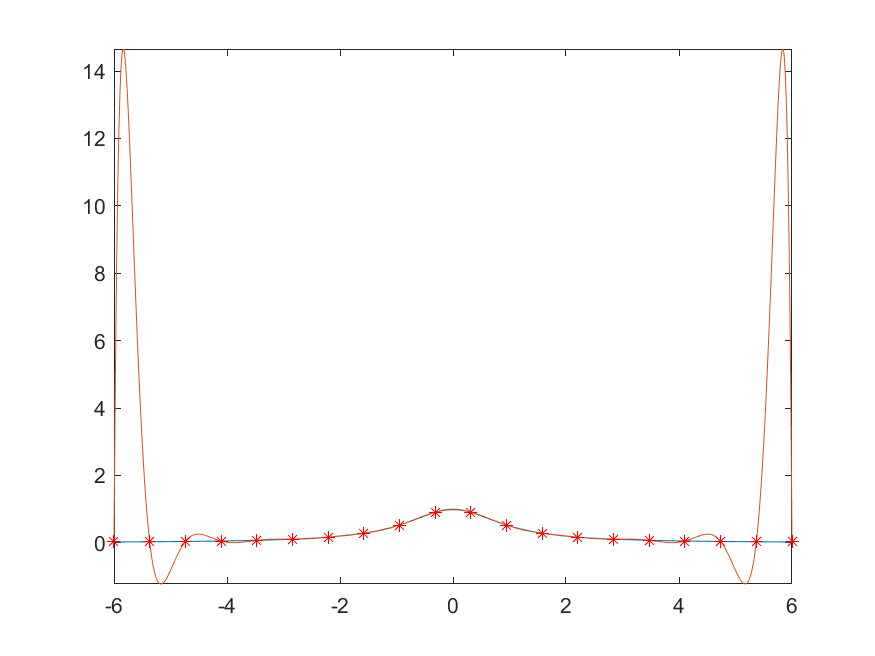
\includegraphics[scale=0.5]{cap4/4_9/20.png} \\

\hspace{3.5cm}\(n=22\) &  \(n=24\) \\
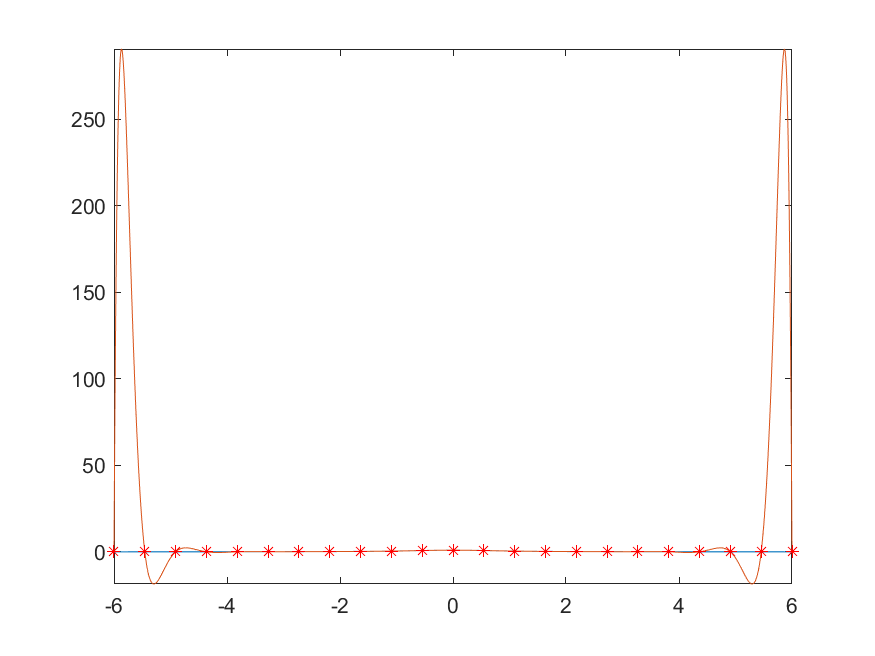
\includegraphics[scale=0.5]{cap4/4_9/22.png} &  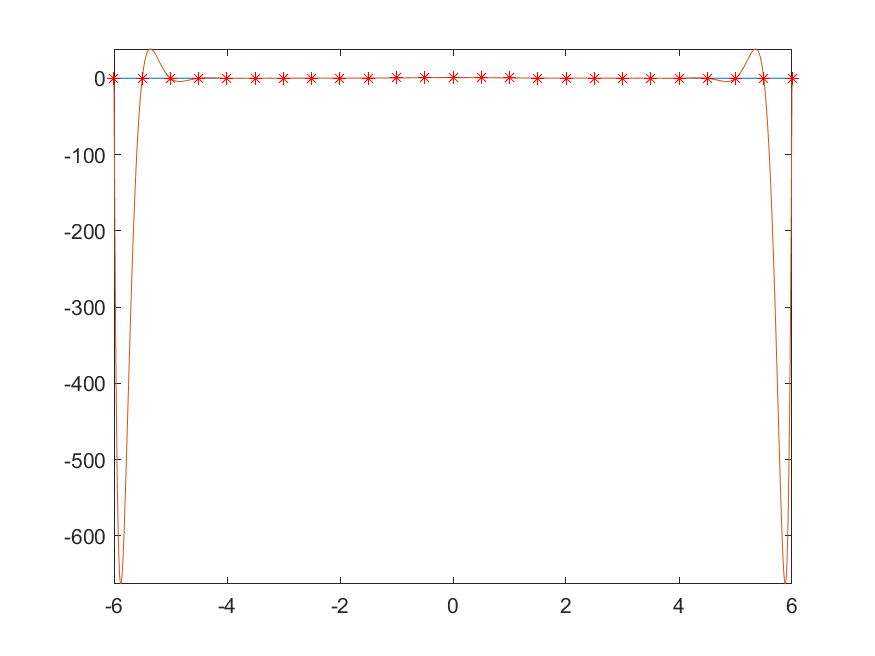
\includegraphics[scale=0.5]{cap4/4_9/24.png} \\

\hspace{3.5cm}\(n=26\) &  \(n=28\) \\
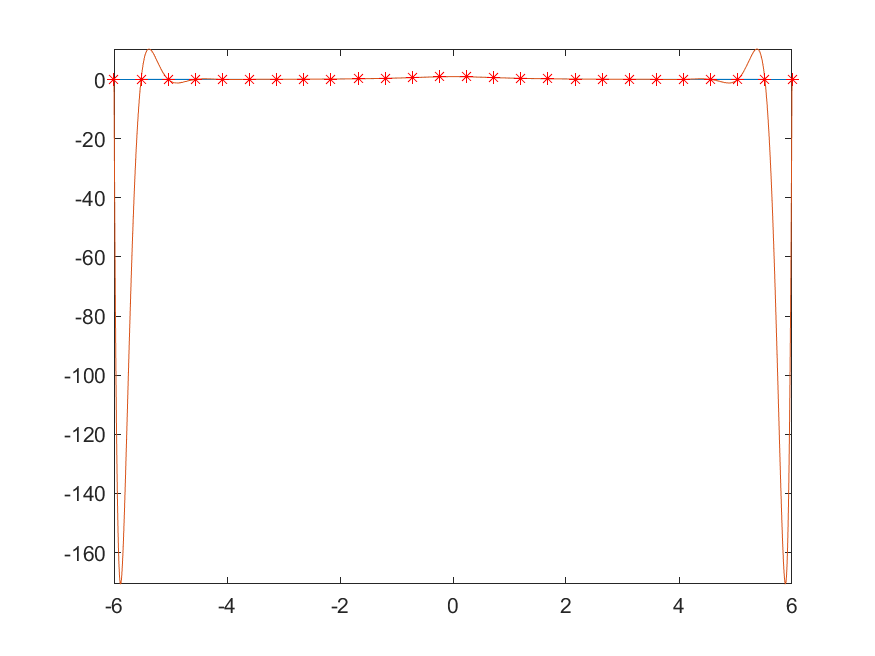
\includegraphics[scale=0.5]{cap4/4_9/26.png} &  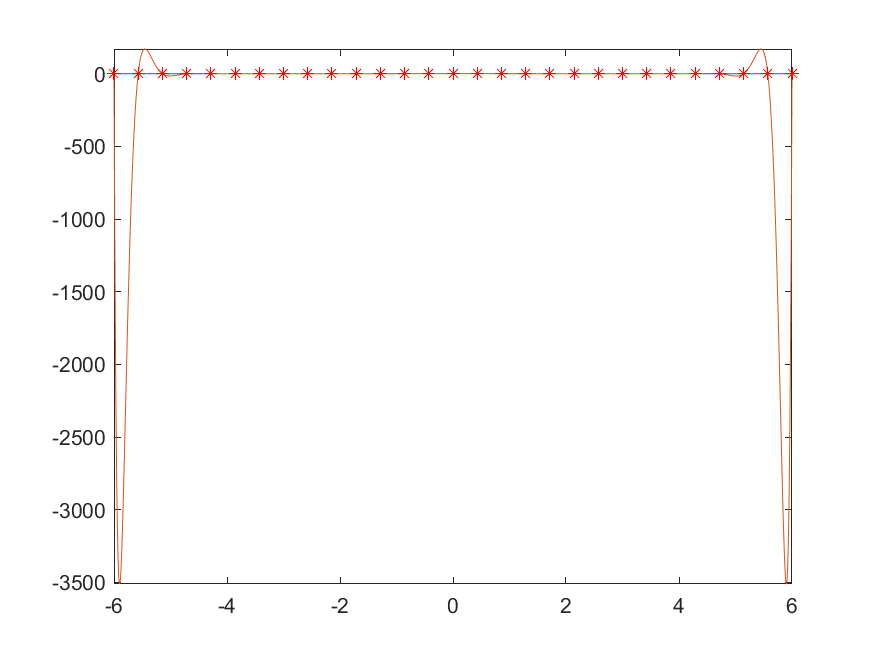
\includegraphics[scale=0.5]{cap4/4_9/28.png} \\
\end{tabular}

\small\begin{tabular}{l*{5}{c}}
\hspace{3.5cm}\(n=30\) &  \(n=32\) \\
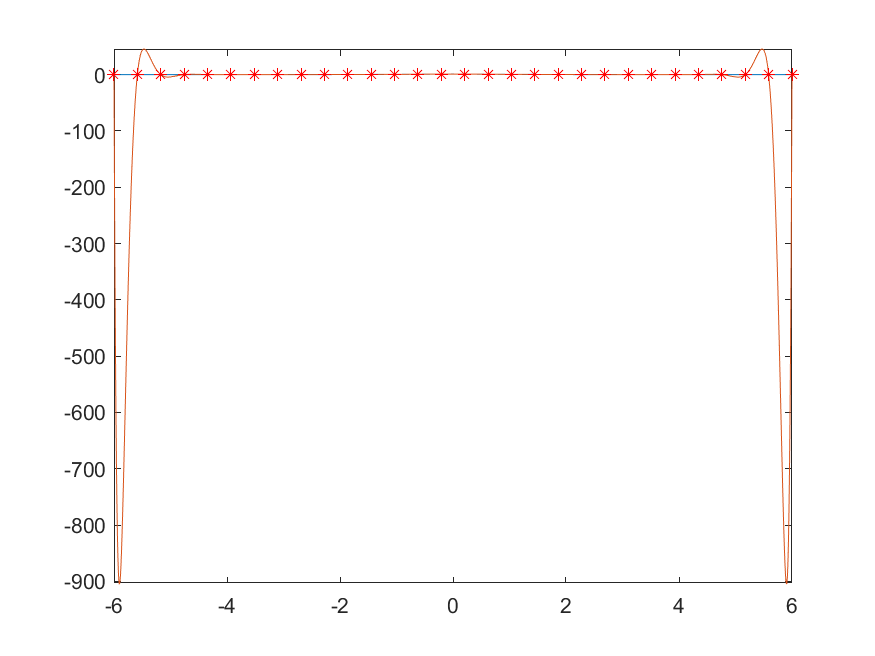
\includegraphics[scale=0.5]{cap4/4_9/30.png} &  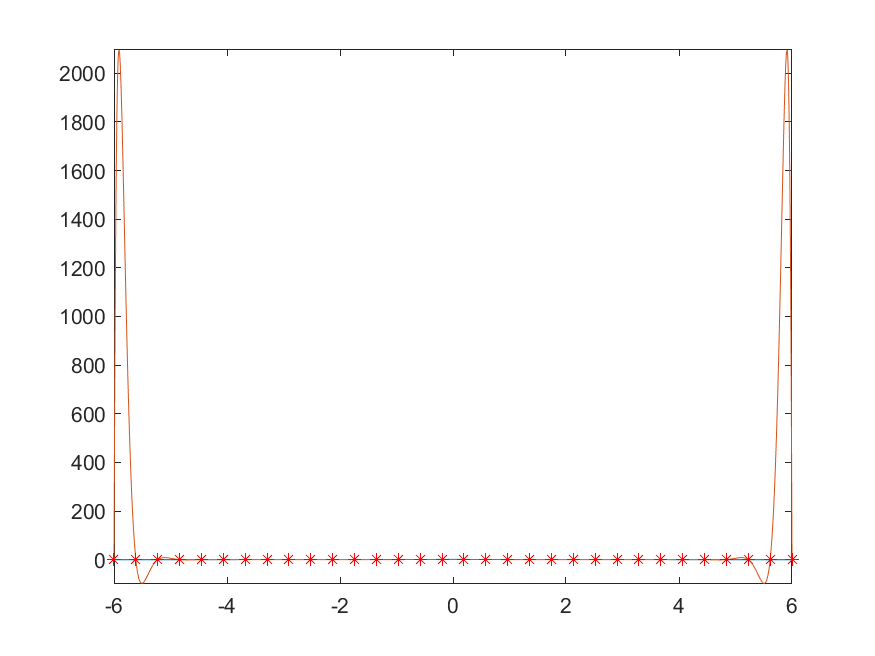
\includegraphics[scale=0.5]{cap4/4_9/32.png} \\

\hspace{3.5cm}\(n=34\) &  \(n=36\) \\
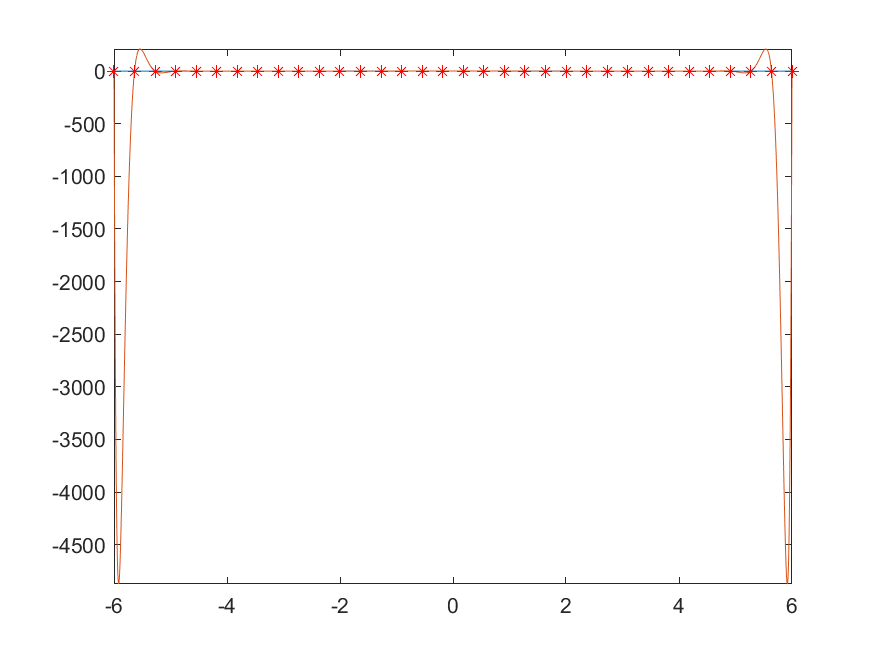
\includegraphics[scale=0.5]{cap4/4_9/34.png} &  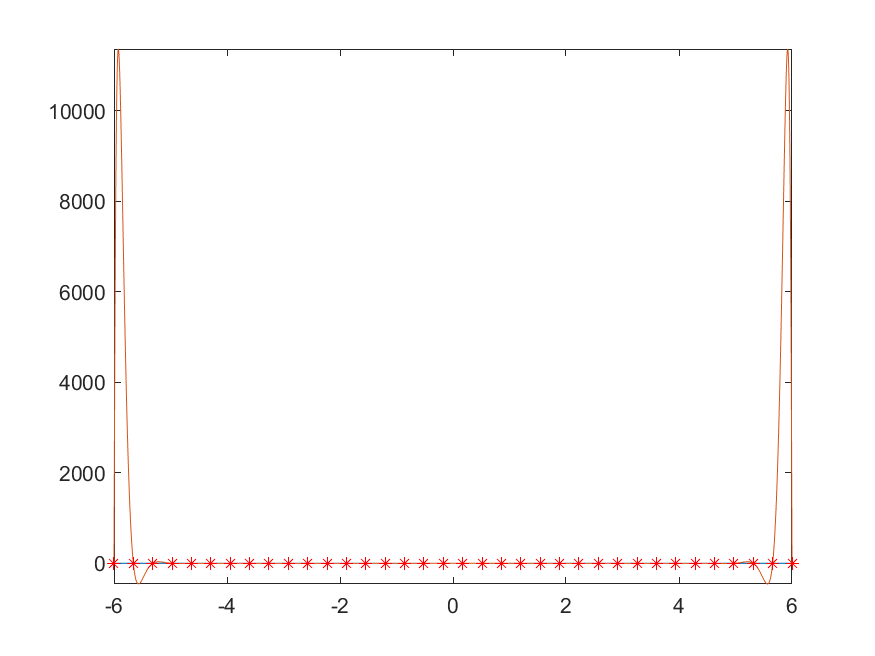
\includegraphics[scale=0.5]{cap4/4_9/36.png} \\

\hspace{3.5cm}\(n=38\) &  \(n=40\) \\
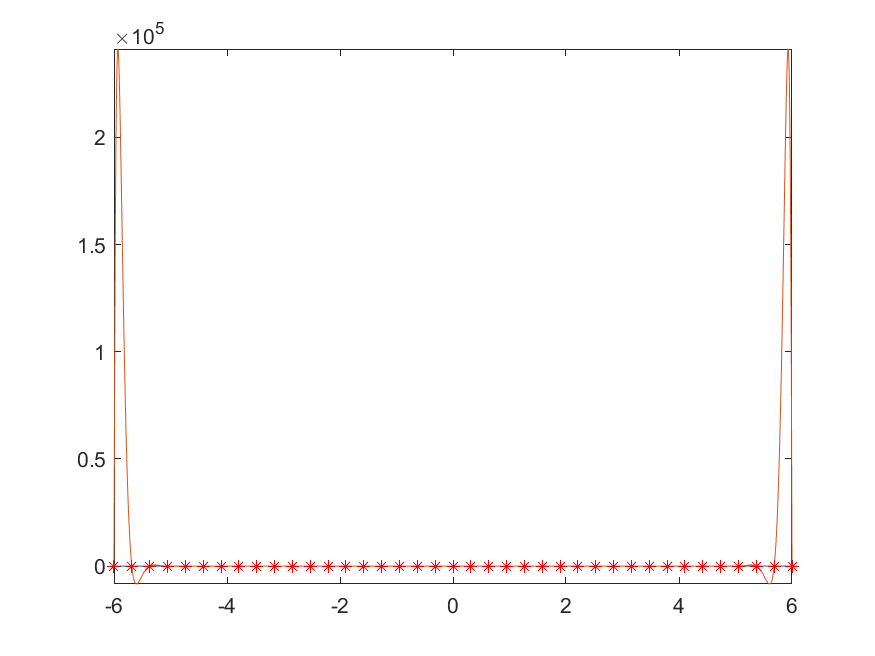
\includegraphics[scale=0.5]{cap4/4_9/38.png} &  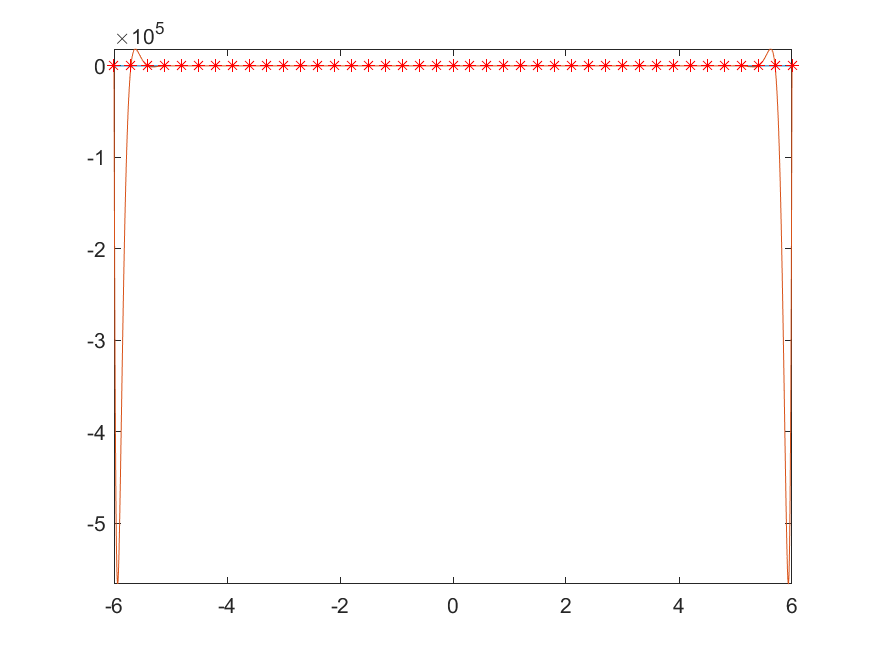
\includegraphics[scale=0.5]{cap4/4_9/40.png} \\
& \\
& \\
& \\
\end{tabular}

\noindent Riguardo alla stima della costante di Lebesgue in funzione di \(n\), abbiamo che:

\[
\Lambda_n \equiv ||\lambda_n|| \text{ con } \lambda_n(x) = \sum^n_{k=0}|L_{k,n}(x)|
\]

\newpage

\noindent Sono state quindi calcolate le stime numeriche mostrate nella seguente tabella:

\begin{center}
	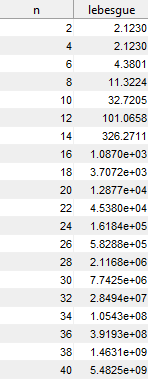
\includegraphics[scale=0.7]{cap4/4_9/4_9.png}
\end{center}

\noindent Inoltre, è stato realizzato anche il seguente grafico mostrante l'andamento dell'errore nell'estremo destro dell'intervallo esmainato. Si noti che \'e stata omessa la parte centrale poich\'e poco interessante, e la parte sinistra dato che l'andamento dell'errore di interpolazione \'e simmetrico rispetto all'asse delle ordinate: questo ha permesso un elevato livello di dettaglio migliorando la chiarezza del grafico.

\begin{center}
	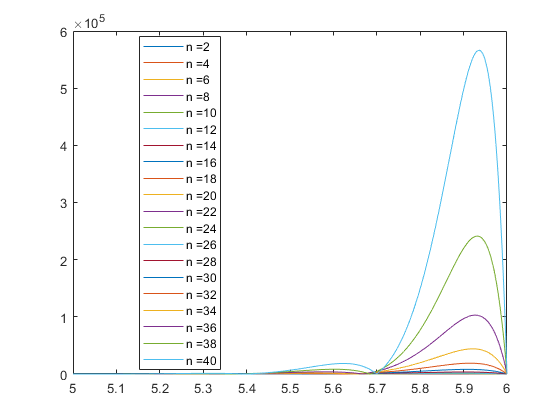
\includegraphics[scale=0.7]{cap4/4_9/4_9_error_plot.png}
\end{center}

\noindent Come si può vedere, all'aumentare di $n$ l'errore aumenta a causa della scelta delle ascisse equispaziate. \\

\noindent Di seguito \'e riportato il codice Matlab con cui sono stati realizzati i grafci e la tabella mostrati. \\

\newpage

\lstinputlisting[language=Matlab]{cap4/4_9.m}

\newpage
\subsection{\textbf{Esercizio 10}}
\begin{center}
\footnotesize\noindent\fbox{
	\parbox{\textwidth}{
	Stimare, nel senso dei minimi quadrati, posizione, velocit\'a iniziale ed accelerazione relative ad un moto rettilineo uniformemente accelerato per cui sono note le seguenti misurazioni dele coppie \((tempo, spazio)\):\\
	\((1, 2.9) \quad (1, 3.1)\quad (2, 6.9) \quad (2, 7.1) \quad (3, 12.9) \quad (3, 13.1) \quad (4, 20.9) \quad (4, 21.1) \quad (5, 30.9) \quad (5, 31.1)\)
	}
}\end{center}

\newpage


\newpage
\section{\textbf{Capitolo 5}}
\vspace{0.8cm}
\subsection{\textbf{Esercizio 1}}
\begin{center}
\footnotesize\noindent\fbox{
	\parbox{\textwidth}{
	  Scrivere una function Matlab che implementi la formula composita dei trapezi su \(n+1\) ascisse equidistanti nell'intervallo \([a, b]\) relativamente alla funzione implementata da \lstinline[language=Matlab]{fun(x)}. \\ \\ La function deve essere del tipo \lstinline[language=Matlab]{If = trapcomp(a, b, fun, tol)}.
}
}\end{center}

\noindent Il seguente codice Matlab implementa la function richiesta. Non sono stati scritti test, in quanto la function verr\'a utilizzata nell'Esercizio 5, seppure in versione leggermente modificata. \\

\lstinputlisting[language=Matlab]{cap5/5_1.m}


\newpage
\subsection{\textbf{Esercizio 2}}
\begin{center}
\footnotesize\noindent\fbox{
	\parbox{\textwidth}{
    Scrivere una function Matlab che implementi la formula composita di Simpson su \(2n+1\) ascisse equidistanti nell'intervallo \([a, b,]\) relativamente alla funzione implementata da \lstinline[language=Matlab]{fun(x)}. \\ \\ La function deve essere del tipo \lstinline[language=Matlab]{If = simpcomp(a, b, fun, tol)}.
}
}\end{center}

\noindent Il seguente codice Matlab implementa la function richiesta. \\

\lstinputlisting[language=Matlab]{cap5/5_2.m}


\newpage
\subsection{\textbf{Esercizio 3}}
\begin{center}
\footnotesize\noindent\fbox{
	\parbox{\textwidth}{
	  Scrivere una function Matlab che implementi la formula composita dei trapezi adattativa nell'intervallo \([a, b]\) relativamente alla funzione implementata da \lstinline[language=Matlab]{fun(x)} e con tolleranza \lstinline[language=Matlab]{tol}. \\ \\ La function deve essere del tipo \lstinline[language=Matlab]{If = trapad(a, b, fun, tol)}.
}
}\end{center}

\noindent Il seguente codice Matlab implementa la function richiesta. \\

\lstinputlisting[language=Matlab]{cap5/5_3.m}


\newpage
\subsection{\textbf{Esercizio 4}}
\begin{center}
\footnotesize\noindent\fbox{
	\parbox{\textwidth}{
	  Scrivere una function Matlab che implementi la formula composita di Simpson adattativa nell'intervallo \([a, b]\) relativamente alla funzione implementata da \lstinline[language=Matlab]{fun(x)} e con tolleranza \lstinline[language=Matlab]{tol}. \\ \\ La function deve essere del tipo \lstinline[language=Matlab]{If = simpad(a, b, fun, tol)}.
}
}\end{center}

\noindent Il seguente codice Matlab implementa la function richiesta. anche in questo caso, riguardo ai test rimane valido quanto detto per gli eserczi precedenti.\\

\lstinputlisting[language=Matlab]{cap5/5_4.m}

\newpage
\subsection{\textbf{Esercizio 5}}
\begin{center}
\footnotesize\noindent\fbox{
	\parbox{\textwidth}{
Calcolare quante valutazioni di funzione sono necessarie per ottenere una approssimazione di 
\[I(f) = \int_0^1 \exp(-10^6 x) dx \] 
che vale \(10^-6\) in doppia precisione IEEE, con una tolleranza \(10^-9\), utilizzando le functions dei precedenti esercizi. Argomentare quantitativamente la risposta.
} }
\end{center}

\noindent Utilizzando versioni leggermente modificate delle function realizzate peri precedenti esercizi, sono stati calcolati i segueni valori:

\begin{itemize}

  \item \textbf{formula composita dei trapezi con \(n+1\) ascisse equidistanti} \\ con \(n=10^7\), \(10^7 +1\) valutazioni di \(\exp(-10^6 x)\), errore pari a \(8.3319 \times 10^{-10}\)
  \item \textbf{formula composita di Simpson su \(2n+1\) ascisse equidistanti } \\ con \(n=2 \times 10^6\), \(2 \times 10^6 + 2\) valutazioni di \(\exp(-10^6 x)\), errore pari a \(3.3715 \times 10^{-10}\)
  \item \textbf{formula dei trapezi adattativa} \\ \(77823\) valutazioni di \(\exp(-10^6 x)\), errore pari a \(1.1253 \times 10^{-14}\)
  \item \textbf{formula di Simpson adattativa} \\ \(1038\) valutazioni di \(\exp(-10^6 x)\), errore pari a \(1.6470 \times 10^{-14}\)

\end{itemize}

\noindent Come si pu\'o vedere dai risultati, la scelta di ascisse equispaziate si rivela inaedeguata per una funzione come quella presa in esame, che presenta una rapida variazione di valore in una porzione dell'intervallo molto ristretta. Infatti, si riesce a catturare efficacemente questa variazione --- e quindi a raggiungere l'approssimazione richiesta sul risultato dell'integrale definito --- soltanto scegliendo di utilizzare un numero elevatissimo di punti, con conseguente bisogno di valutare moltissime volte la funzione.\\

\noindent Le formule adattive invece performano molto meglio, perch\'e individuano i nodi della partizione in base al comportamento locale della funzione, permettendo quindi di minimizzare l'errore e, di conseguenza, le chiamate ricorsive necessarie al raggiungimento della soglia di tolleranza prestabilita.\\

\noindent Il codice Matlab utilizzato per realizzare quanto descritto sopra \'e il seguente: \\

\lstinputlisting[language=Matlab]{cap5/5_5.m}


\newpage



\newpage
\pagenumbering{roman}
\section{\textbf{Figure}}
%\input{figure.tex}


\end{document}
